\documentclass{article}
\usepackage[T1]{fontenc}
\usepackage[utf8]{inputenc}
\usepackage[polish]{babel}
\usepackage{ragged2e}
\usepackage{blindtext}
\usepackage{graphicx}
\usepackage{geometry}
\usepackage{setspace}
\usepackage{tabulary}
\usepackage{enumitem}
\usepackage{url}
\usepackage{subfig}
\usepackage{float}
\usepackage[ampersand]{easylist}
\usepackage{xcolor}
\usepackage{sectsty}
\usepackage[font=large,labelfont=bf]{caption}
%\usepackage{showframe}

\geometry{left=3cm, right=3cm, top=1.5cm, bottom=1.5cm}
\graphicspath{ {./images/} }

\begin{document}
\begin{titlepage}
    \begin{center}

        \vspace*{1cm}
        
        {
            \LARGE
            Akademia Górniczo Hutnicza\\
            \vspace{0.2cm}
            im. Stanisława Staszica w Krakowie
        }

        \vspace{0.5cm}

        \begin{figure}[h]
            \centering
            
\includegraphics[width=\textwidth]{logo.png}
        \end{figure}

        \vspace{0.5cm}

        {
            \LARGE
            Wydział Inżynierii Metali i Informatyki Przemysłowej\\
            \vspace{0.2cm}
            Katedra Informatyki Stosowanej i Modelowania
        }

        \vspace{0.5cm}

        {
            \LARGE
            Praca Dyplomowa Inżynierska
        }

        \vspace{0.5cm}

        {
            \Large
            \textbf{,,Interaktywne przetwarzanie obrazów mikroskopowych\\
            związanych z oceną adhezji składników komórkowych''}
        }

        \vspace{0.5cm}

        {
            \Large
            \textbf{,,Interactive processing of microscopic images\\
            related to evaluation adhesion of cellular components''}
        }

        \vfill

        \begin{flushleft}
        {
            \Large
            \begin{tabular}{ l l c }
                autor: & Konrad Lenart\\
                kierunek: & Inżynieria Obliczeniowa\\
                opiekun pracy: & dr hab. Magdalena Kopernik
            \end{tabular}
        }
        \end{flushleft}

        \vspace{0.5cm}

        {
            \Large
            Kraków, 2020
        }

        \vspace{1cm}

    \end{center}
\end{titlepage}

\sectionfont{\LARGE}
\subsectionfont{\Large}
\subsubsectionfont{\large}

\setstretch{2.5}
    \newpage
    {
        \Large
        \justifying
        Uprzedzony o odpowiedzialności karnej na podstawie art. 115 ust. 1 i 2 ustawy z dnia 4 lutego
        1994 r. o prawie autorskim i prawach pokrewnych (tj. Dz.U. z 2006 r. Nr 90, poz. 631 z późn.
        zm.): „Kto przywłaszcza sobie autorstwo albo wprowadza w błąd co do autorstwa całości lub
        części cudzego utworu albo artystycznego wykonania, podlega grzywnie, karze ograniczenia
        wolności albo pozbawienia wolności do lat 3. Tej samej karze podlega, kto rozpowszechnia bez
        podania nazwiska lub pseudonimu twórcy cudzy utwór w wersji oryginalnej albo w postaci
        opracowania, artystyczne wykonanie albo publicznie zniekształca taki utwór, artystyczne
        wykonanie, fonogram, wideogram lub nadanie.”, a także uprzedzony o odpowiedzialności
        dyscyplinarnej na podstawie art. 211 ust. 1 ustawy z dnia 27 lipca 2005 r. Prawo o szkolnictwie
        wyższym (tj. Dz. U. z 2012 r. poz. 572, z późn. zm.) „Za naruszenie przepisów obowiązujących
        w uczelni oraz za czyny uchybiające godności studenta student ponosi odpowiedzialność
        dyscyplinarną przed komisją dyscyplinarną albo przed sądem koleżeńskim samorządu
        studenckiego, zwanym dalej „sądem koleżeńskim”, oświadczam, że niniejszą pracę
        dyplomową wykonałem osobiście, samodzielnie, i że nie korzystałem ze źródeł innych niż
        wymienione w pracy.
    }

    \vfill

    \begin{center}
        {
            \Large
            \setstretch{1.0}
            \setlength{\tabcolsep}{2em}
            \begin{tabulary}{0.75\textwidth}{ c c c }
                Kraków, dnia........................ && ................................\\
                (miejscowość)& & (podpis)\\
            \end{tabulary}
        }
    \end{center}
    
    \newpage
    \begin{center}
        {
            \Large
            \setstretch{1.0}
            \tableofcontents
        }
    \end{center}
    \newpage
    
    \section{Wstęp}
    \setstretch{1.5}
    {
        \Large
        \justifying
        \quad 
        Każdy dzień to nowy rekord postępu dla całej cywilizacji technicznej.
        Szybkość z jaką pojawiają się nowe technologie stale rośnie.
        Nikogo nie dziwi już ile ludzkość potrafi dokonać w ciągu dwudziestu czterech godzin.
        Obecny trend rozwoju zawdzięczamy pojawieniu się komputerów.
        Komputery zastąpiły ludzi w wielu czynnościach, stworzyły także nowe miejsca pracy.
        Wyreczają nas w skomplikowanych obliczeniach, pozwalają testować systemy bezpieczeństwa w samochodach bez konieczności ich niszczenia, nauczyliśmy je nawet pilotować olbrzymie samoloty.
        Każdy z nas nosi w kieszeni większą moc obliczeniową niż komputery obecne na statkach kosmicznych, które lądowały na księżycu w ramach programu Apollo.
        Zaprzęgnięcie komputerów do automatyzacji pracy, którą ludzie do tej pory wykonywali ręcznie zaoszczędza nam sporo czasu.
        Charakter tej pracy jest analogiczny - zastąpienie ludzi w mozolej, ręcznej ocenie adhezji składników komórkowych -
        automatycznym procesem, który przez człowieka będzie tylko nadzorowany.
    }
    
    \vspace{0.5cm}
    \setstretch{1.5}
    {
        \Large
        \justifying
        Jedną z najważniejszych dziedzin, w której komputery znalazły zastosowanie jest medycyna.
        Postęp w tej dziedzinie ratuje każdego dnia miliony istnień na całym świecie.
        W niniejszej pracy podjęto próbę oceny adhezji składników komórkowych wykorzystując do tego analizę i przetwarzanie obrazów cyfrowych pochodzących z mikroskopu.
        Z pomocą odpowiednich algorytmów zliczone zostają obiekty widoczne na zdjęciu.
        Następnie bazując na faktach o składnikach komórkowych krwii obiekty zostają zakwalifikowane jako komórka krwii lub odrzucone.
    }

    \vspace{0.5cm}
    \setstretch{1.5}
    {
        \Large
        \justifying
        Założeniem pracy było stworzenie łatwej w obsłudze biblioteki napisanej w języku C++.
        Biblioteka napisana została w taki sposób, aby z łatwością można było dołączyć ją do istniejących projektów w środowisku Visual Studio.
        Cele poboczne pracy to stworzenie interfejsu użytkownika w celu zaprezentowania funkcjonalności bibilioteki.
        Do tego celu wykorzystana została aplikacja na komputery osobiste z wykorzystaniem .NET Framework 4.7.2.
        Dokładny opis biblioteki jak i interfejsu użytkownika ma miejsce w rozdziale drugim po części teoretycznej, traktującej o wszystkich wykorzystanych w programie zagadnieniach związanych z analizą i przetwarzaniem obrazów cyfrowych.
    }

    \vfill

    \newpage
    \section{Cele i założenia}
        \subsection{Cel główny}
        \setstretch{1.5}
        {
            \Large
            \justifying
            \quad
            Celem głównym było stworzenie biblioteki zajmującej się analizą i przetwarzaniem obrazów cyfrowych.
            Biblioteka ma za zadanie ocenę adhezji komórek krwi widocznych na obrazach pochodzących z mikroskopu, ma również ułatwić oraz usprawnić pracę ludzi.
            Podczas pracy nad biblioteką utrzymywany był kontakt z osobami, które będą z niej korzystać.
            Biblioteka napisana została w taki sposób, aby dostosować jej funkcjonalności do istniejącej już metodologii.
            Dzięki temu analiza obrazów niosących informacje na temat krwi pozwoli zaoszczędzić znaczącą ilość czasu.
        }
        \subsection {Cel poboczny}
        \setstretch{1.5}
        {
            \Large
            \justifying
            \quad
            Celem pobocznym było stworzenie interatywnej aplikacji okienkowej, w której zaprezentowane zostało działanie biblioteki.
            Aplikacja służy zaprezentowaniu procesów zachodzących podczas analizy i przetwarzania obrazów cyfrowych.
            Pozwala również na interakcje z procesem, jego zmianę, zatrzymanie, dostosowanie parametrów oraz podgląd tego co się dzieje w czasie rzeczywistym.
            Do tego celu zostały wykorzystane następujące technologie: C++/CLI, C\#, Windows Presentation Foundation oraz .NET Framework 4.7.2.
        }
        \subsection{Założenia}
        \setstretch{1.5}
        {
            \Large
            \justifying
            \quad
            Głównym założeniem tworzonego oprogramowania było stworzenie biblioteki w taki sposób, aby osoby z niej korzystające z łatwością mogły dodać ją do swoich projektów w środowisku Visual Studio 2019.
            Funkcjonalności jakie niesie ze sobą nie skupiają się wyłącznie na analizie i przetwarzaniu obrazów cyfrowych.
            Biblioteka dba również o to, aby struktura folderów była w należytym stanie na podstawie głównego folderu.
            Główny folder powinien gromadzić kolejne foldery, tak zwane eksperymenty, gdzie przez eksperyment rozumiemy folder, w którym znajdują się dane pochodzące z mikroskopu.
            W każdym z takich folderów dodane zostają odpowiednie pliki odpowiedzalne za ustawienia.
            Jeżeli dany eksperyment posiada już plik ustawień, jest to jasny sygnał dla programu, że nie należy dodawać kolejnego.
        }

        \newpage
        \setstretch{1.5}
        \subsection{Podstawowe funkcje biblioteki}
        {
            \Large
            \quad
            \begin{enumerate}
                \color{blue}
                {
                \item Analiza drzewa folderów,
                \item Zliczanie komórek krwi na obrazach cyfrowych,
                \item Zapis wyniku pracy algorytmu zliczającego liczbę komórek krwi w ramach eksperymentu do pliku,
                \item Uruchomienie procesu przygotowania katalogu głównego w sposób asynchroniczny,
                \item Uruchomienie procesu przetwarzania obrazów w sposób asynchroniczny,
                \item Logowanie wykonywanych operacji,
                \item Personalizacja procesu przetwarzania danego obrazu przez wybranie operacji, które będą na nim wykonane.
                }
            \end{enumerate}
        }

        \subsection{Podstawowe funkcje aplikacji okienkowej}
        {
            \Large
            \quad
            \begin{enumerate}
                \color{blue}
                {
                \item Podgląd obrazów, które powstały po podzieleniu obrazu głównego,
                \item Podgląd obrazu, powstałego w procesie binaryzacji,
                \item Możliwość śledzenia algorytmu przetwarzania obrazów w czasie rzeczywistym,
                \item Możliwość śledzenia algorytmu przygotowania katalogu głownego w czasie rzeczywistym,
                \item Możliwość zatrzymania procesów: przetwarzania obrazów oraz przygotowania katalogu głownego.
                }
            \end{enumerate}
        }

        \setstretch{1.5}
        \subsection{Rekomendacje}
        {
            \Large
            \justifying
            \quad
            Użytkownikom oprogramowania rekomenduje sie wykorzystywanie biblioteki na systemie operacyjnym Windows 10 w projektach budowanych z wykorzystaniem MSBuild (Microsoft Build Engine) w konfiguracji 32 lub 64-bitowej \cite{msdocsmsbuild}.
        }

    \section{Część teoretyczna}
        \subsection{Adhezja komórek}
        {
            \label{sec:adhezja-komorek}
            \Large
            \justifying
            \quad
            Adhezja komórek - to proces, w którym komórki za pomocą cząsteczek znajdujących się w błonie komórkowej, oddziałują między sobą, co umożliwa ich przyleganie.
            Interakcja między komórkami zachodzi dzięki białkom błony należącymi do grupy cząsteczek adhezyjnych CAMs \textit{cell-adhesion molecules} (w tym kadheryny, selektyny, integryny, nadrodzina immunoglobulin), umożliwia tworzenie połączeń miedzykomórkowych i ich przyleganie
            \cite{Molecular Biology of the Cell. 4th edition}.
            Adhezja, z łac. \textit {adhaesio} oznacza \textit{przyleganie} \cite{adhezja}, w kontekscie tej pracy mówimy o większej adhezji, gdy więcej komórek znajduje się na obrazie.
            Analogicznie mniejsza adhezja oznacza mniejszą liczbę komórek.
        }
        \subsection{Rozszerzenie TIFF}
        {
            \label{sec:rozszerzenie-tiff}
            \Large
            \justifying
            \quad
            TIFF - \textit{Tag Image File Format} jest to format plików służący do przechowywania obrazów rastrowych.
            TIFF ma bardzo szerokie zastosowania, od urzadzeń służących do skanowania czy wysyłania faksów do analizy i przetwarzania obrazów cyfrowych.
            Format stworzony przez \textit{Aldus Corporation}, nieistniejącego już dzisiaj przedsiębiorstwa przejętego w 1994 przez \textit{Adobe}.
            TIFF jest elastycznym i adaptatywnym typem plików służącym do przechowywania zdjęć bez utraty ich jakości.
            Dzięki temu, że przechowywane dane nie tracą jakości, TIFF jest używany do archiwizacji zdjęć, ponieważ w przeciwieństwie do rozszerzenia JPEG,
            TIFF może być zmieniany i zapisywany wielokrotnie bez utraty jakości obrazu.
            Rozszerzenie to niesie ze sobą możliwość pracy zarówno wykorzystując kolory z palety RGB czy też monochromatyczne.
            Jest to bardzo użyteczny format, szczególnie w kontekscie analizy i przetwarzania obrazów cyfrowych \cite{Encyclopedia of Graphics File Formats: The Complete Reference}.
        }
        \subsection{Binaryzacja}
        {
            \label{sec:binaryzacja}
            \Large
            \justifying
            \quad
            Binaryzacja - służy do stworzenia nowego obrazu na podstawie innego w taki sposób, aby zaznaczyć interesujący nas fragment na czarno(białe tło)
            lub na biało(czarne tło). Jak sama nazwa wskazuje wartości w nowym obrazie są 0 lub 1. Dzięki binaryzacji jesteśmy w stanie przetwarzać obraz
            tylko dla fragmentów zaznaczonych w procesie binaryzacji. Binaryzację można przeprowadzać na przykład na podstawie wartości kolorów w poszczególnych
            macierzach RGB. Na przykład: 
            jeżeli \(czerwony > 150\), \(zielony > 200\) i \(niebieski < 122\) to wartość danego pixela w nowym obrazie równa się 1.
            Teraz wystarczy zastosować to dla każdego piksela w obrazie wejściowym i naszym obrazem wyjściowym staje się obraz o tym samym rozmiarze
            z zaznaczonym na czarno obszarem, gdzie macierze RGB miały wartości \(czerwony > 150\), \(zielony > 200\) i \(niebieski < 122\).
            Tak więc, gdy dokonamy już binaryzacji jesteśmy gotowi do kolejnych działań.
            Takich jak na przykład etykietowanie, erozja, dylatacja, otwarcie, zamkniecie czy innego rodzaju operacje morfologiczne \cite{Digital Image Processing Second Edition}.
        }
        \subsection{Element Strukturalny}
        {
            \label{sec:element-strukturalny}
            \Large
            \justifying
            \quad
            Element Strukturalny - operacje morfologiczne opierają się na elemencie strukturalnym.
            Przez element strukturalny należy rozumieć ruchome okno, które przykładane jest do każdego piksela w obrazie.
            Na podstawie wartości w sąsiedztwie wykonywane są pewne operacje.
            Po przyłożeniu punktu centralnego do piksela, sprawdzana jest wartość tego piksela.
            Jeżeli wartość ta jest równa \(1\) to zazwyczaj oznacza to aktywację.
            Na przykład zamalowanie odpowiednich sąsiadów danego piksela zgodnie z tym, jak wygląda element strukturalny.
            Każdy z punktów elementu strukturalnego ma odpowiednią wartość.
            Punkt centralny punktu strukturalnego to miejsce, które przykłada się do kolejnych pikseli w obrazie binarnym, w zależności od operacji morfologicznej, która jest przeprowadzana.
            Pozostałe piksele przyjmują jakąś wartość \(0\) lub \(1\).
            Przykłady elementów strukturalnych (granatowym kolorem zaznaczono punkty centralne, szarym wartość \(1\), białym wartość \(0\)) przedstawiono na Rysunkach od \ref{elementy_strukturalne} \cite{Digital Image Processing Second Edition}.
        }

        \begin{figure}[H]
            \centering
            \subfloat[\centering]{{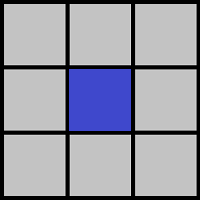
\includegraphics[width=90px]{element_strukturalny_1.png}}}
            \qquad
            \subfloat[\centering]{{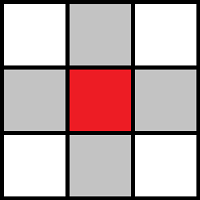
\includegraphics[width=90px]{element_strukturalny_2.png}}}
            \qquad
            \subfloat[\centering]{{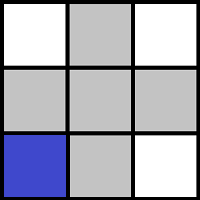
\includegraphics[width=90px]{element_strukturalny_3.png}}}
            \qquad
            \subfloat[\centering]{{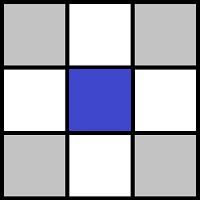
\includegraphics[width=90px]{element_strukturalny_4.png}}}
            \qquad
            \subfloat[\centering]{{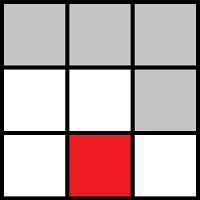
\includegraphics[width=90px]{element_strukturalny_5.png}}}
            \caption{(\textit{Opracowanie własne}) Element Strukturalny.
            (a) Przykład elementu strukturalnego o rozmiarze \(3 \times 3\) z punktem centralnym w środku.
            Wszystkie piksele elementu strukturalnego posiadają wartość równą 1.\\
            (b) Przykład elementu strukturalnego o rozmiarze \(3 \times 3\) z punktem centralnym w środku.
            Lewy dolny, lewy górny, prawy dolny oraz prawy górny piksel posiada wartość 0.\\
            (c) Przykład elementu strukturalnego o rozmiarze \(3 \times 3\) z punktem centralnym w lewym dolnym rogu.
            Lewy górny, prawy górny oraz prawy dolny piksel posiada wartość 0.\\
            (d) Przykład elementu strukturalnego o rozmiarze \(3 \times 3\) z punktem centralnym w środku.
            Lewy środkowy, prawy środkowy, dolny środkowy oraz górny środkowy piksel posiada wartość 0.\\
            (e) Przykład elementu strukturalnego o rozmiarze \(3 \times 3\) z punktem centralnym w dolnym środkowym pikselu.
            Lewy dolny, lewy środkowy, środkowy oraz prawy dolny piksel mają wartość równą 0.}
            \label{elementy_strukturalne}
        \end{figure}

        \subsection{Sąsiedztwo}
        {
            \label{sec:sasiedztwo}
            \Large
            \justifying
            \quad
            Sąsiedztwo - jest to sposób w jaki zdefiniowane jest otoczenie danego piksela.
            Wyróżnia się dwa głowne sąsiedztwa: Moore'a (Rysunek \ref{neighbourhood}(a)) oraz Von Neumann'a (Rysunek \ref{neighbourhood}(b)) \cite{Digital Image Processing Second Edition}.
        }
        \begin{figure}[H]
            \centering
            \subfloat[\centering]{{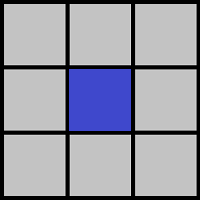
\includegraphics[width=90px]{element_strukturalny_1.png}}}
            \qquad
            \subfloat[\centering]{{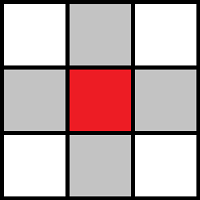
\includegraphics[width=90px]{element_strukturalny_2.png}}}
            \caption{(\textit{Opracowanie własne}) (a) Sąsiedztwo Moore'a. (b) Sąsiedztwo Von Neumann'a.}
            \label{neighbourhood}
        \end{figure}

        \subsection{Erozja}
        {
            \label{sec:erozja}
            \Large
            \justifying
            \quad
            Erozja - czyli zwężanie, to przyłożenie elementu strukturalnego do każdego piksela \(p_{ij}\) na obrazie w celu sprawdzenia czy choć jeden piksel z sąsiedztwa \(p_{ij}\) ma wartość równą zero.
            Jeżeli tak, to punkt centralny również przyjmuje wartość 0. W przeciwnym przypadku wartość pozostaje bez zmian \cite{Digital Image Processing Second Edition}.
        }

        \begin{figure}[H]
            \centering
            \subfloat[\centering]{{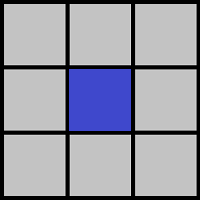
\includegraphics[width=90px]{element_strukturalny_1.png}}}
            \qquad
            \subfloat[\centering]{{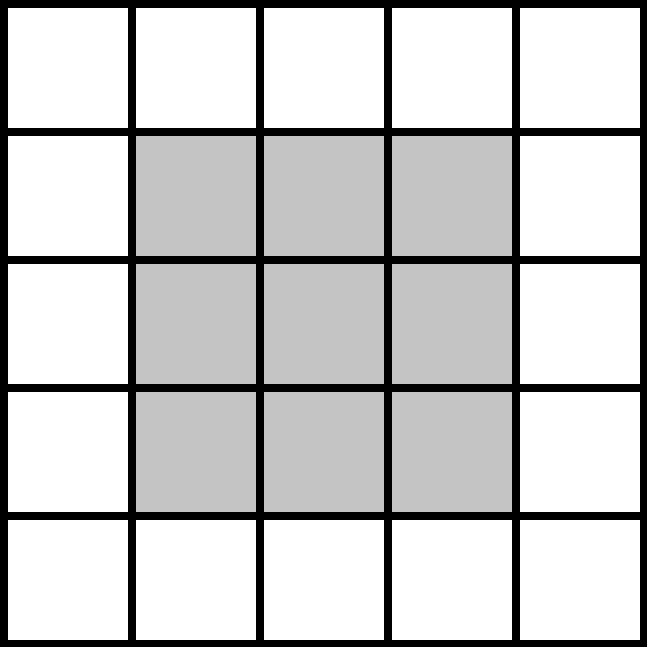
\includegraphics[width=90px]{przed_erozja.png}}}
            \qquad
            \subfloat[\centering]{{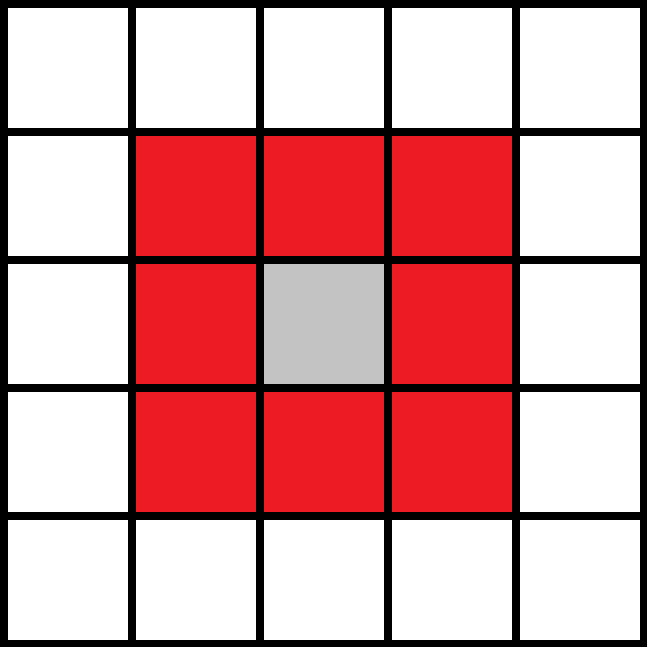
\includegraphics[width=90px]{po_erozji.png}}}
            \caption
            {
                (\textit{Opracowanie własne}) Erozja.
                (a) Element strukturalny użyty w operacji.
                (b) Stan przed erozją z wykorzystaniem elementu strukturalnego z podpunktu (a).
                (c) Stan po erozji z wykorzystaniem elementu strukturalnego z podpunktu (a).
                Granatowym kolorem zaznaczono punkt centralny elementu strukturalnego, natomiast czerwonym piksele, które zmieniły wartości z 1 na 0.
            }
            \label{erozja}
        \end{figure}

        \subsection{Dylatacja}
        {
            \label{sec:dylatacja}
            \Large
            \justifying
            \quad
            Dylatacja - czyli rozszerzanie, polega na przyłożeniu elementu strukturalnego do każdego piksela \(p_{ij}\) na obrazie w celu sprawdzenia czy choć jeden z pikseli z sąsiedztwa \(p_{ij}\) ma wartość równą jeden.
            Jeżeli tak, to punkt centralny również przyjmuje wartość 1, w przeciwnym wypadku wartość nie ulega zmianie \cite{Digital Image Processing Second Edition}.
        }

        \begin{figure}[H]
            \centering
            \subfloat[\centering]{{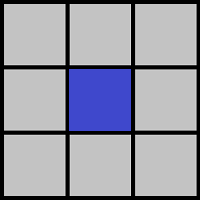
\includegraphics[width=90px]{element_strukturalny_1.png}}}
            \qquad
            \subfloat[\centering]{{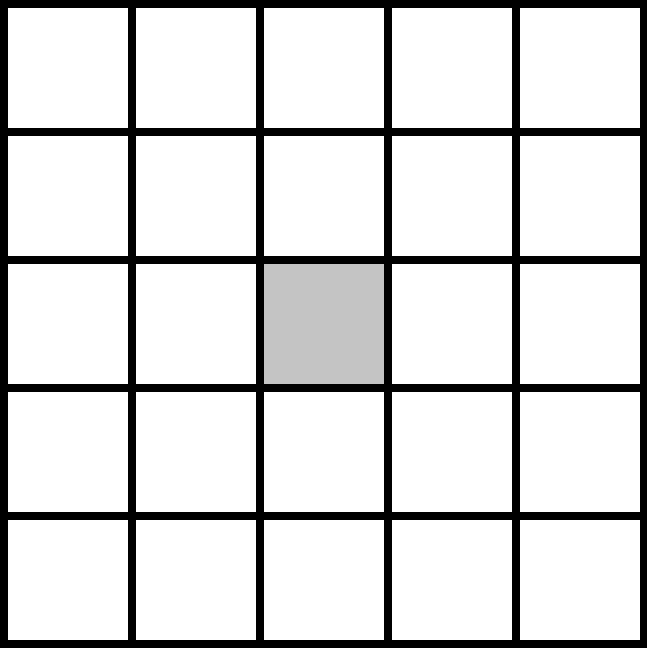
\includegraphics[width=90px]{przed_dylatacja.png}}}
            \qquad
            \subfloat[\centering]{{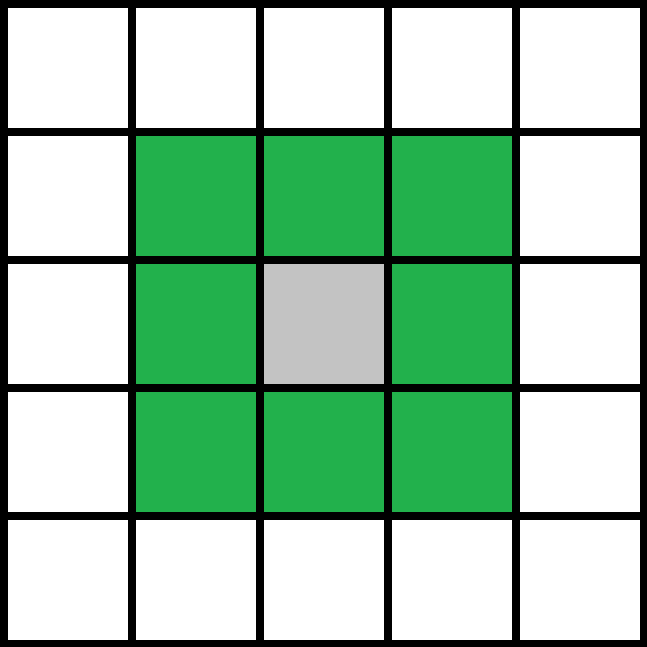
\includegraphics[width=90px]{po_dylatacji.png}}}
            \caption
            {
                (\textit{Opracowanie własne}) Dylatacja.
                (a) Element strukturalny użyty w operacji.
                (b) Stan przed dylatacją z wykorzystaniem elementu strukturalnego z podpunktu (a).
                (c) Stan po dylatacji z wykorzystaniem elementu strukturalnego z podpunktu (a).
                Granatowym kolorem zaznaczono punkt centralny elementu strukturalnego, natomiast zielonym piksele, które zmieniły wartości z 0 na 1.
            }
            \label{dylatacja}
        \end{figure}

        {
            \Large
            \justifying
            \quad
            Dylatacja i erozja są operacjami dualnymi.
            Oznacza to, że jeżeli wykonamy negatyw obrazu, a nastepnie zadziałamy identycznym elementem strukturalnym na negatyw, to skutkiem takich działań będzie odwrotność działania erozji z dylatacją.
            Erozja na negatywie zadziała z takim samym skutkiem, jak dylatacja na oryginale.
            Natomiast zastosowanie dylatacji na negatywie przyniesie takie same skutki jak wykonanie erozji na oryginale.
        }

        \vspace{0.5cm}

        {
            \Large
            \justifying
            \quad
            Należy zauważyć, że dylatacja i erozja nie są operacjami odwrotnymi.
            Przykłady powyżej (Rysunek \ref{erozja}, Rysunek \ref{dylatacja}) mogą coś takiego sugerować, jednak tak nie jest.
            Dzięki dylatacji możemy zamykać otwory w obiektach znajdujących się na obrazie.
            Po wykonaniu takiej operacji i zamknięciu obiektu, erozja nie sprawi, że obiekt na nowo się otworzy.
            To samo tyczy się pojedynczych punktów (piksele, których każdy sąsiad ma wartość 0).
            Zadziałanie na taki pojedynczy piksel erozją sprawi, że zmieni on wartość z 1 na 0.
            Nie da się zadziałać dylatacją w taki sposób, aby taki punkt na nowo się pojawił.
            Pozwala to wyciągnąc następujące wnioski:
            Dylatacja jest świetnym sposobem na zamykanie drobnych dziur.
            Erozja jest świetna w usuwaniu małych obiektów.
            Jednak te operacje mają swoje minusy, nie działamy erozją czy dylatacją tylko na wybrane punkty.
            Działamy nimi na cały obraz.
            Właśnie dlatego powstały dwie kolejne operacje: otwarcie oraz zamknięcie.
        }

        \subsection{Otwarcie morfologiczne}
        {
            \label{sec:otwarcie-morfologiczne}
            \Large
            \justifying
            \quad
            Otwarcie morfologiczne - jest równoważne dwom następującym po sobie operacjom na obrazie: erozji, a następnie dylatacji.
            Operacja ta pozwala usunąć małe elementy, tak zwany szum i następnie odbudować te obiekty, które ucierpiały na skutek erozji.
            Dzięki temu uzyskujemy czysty obraz, pozbawiony drobnych obiektów.
            Jak możemy zauważyć na Rysunku \ref{Otwarcie_Morfologiczne}(b), pojedyncze piksele (nie posiadające sąsiadów z wartością 1 zostały usunięte), następnie reszta obiektów zostaje odbudowana \cite{Digital Image Processing Second Edition}.
        }
        \begin{figure}[H]
            \centering
            \subfloat[\centering]{{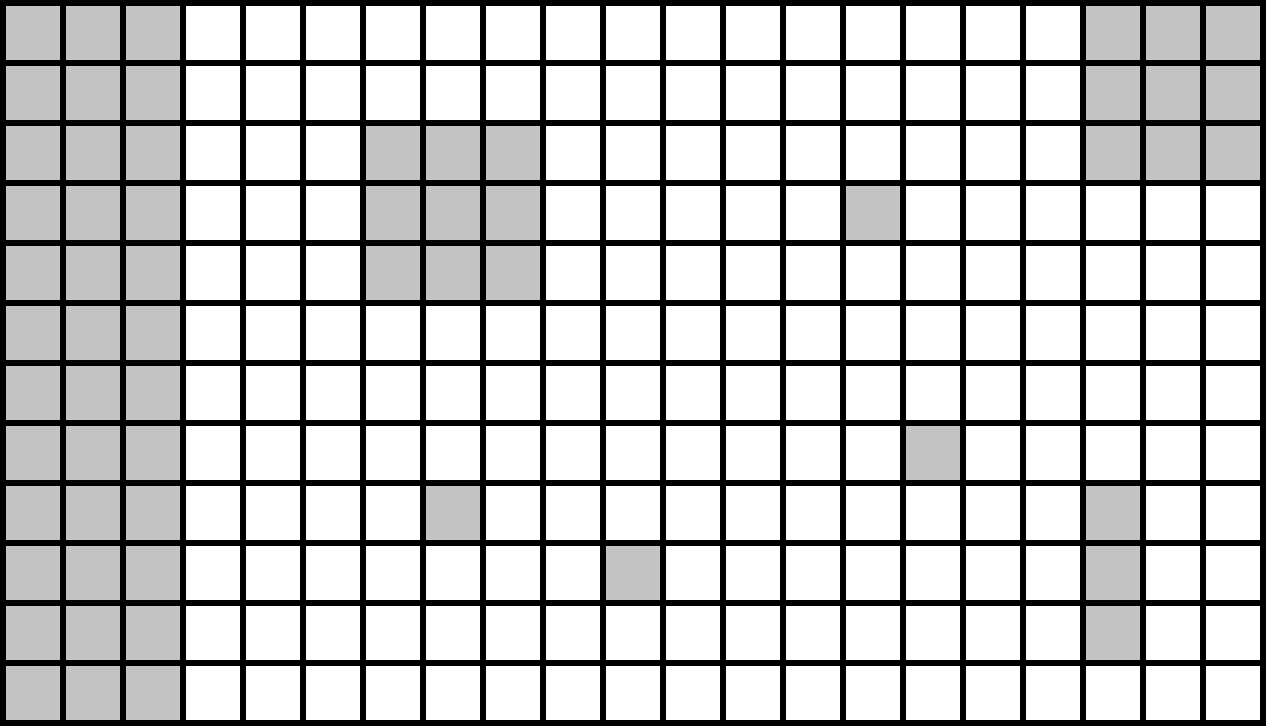
\includegraphics[width=170px]{otwarcie-morfologiczne-stan-poczatkowy.png}}}
            \qquad
            \subfloat[\centering]{{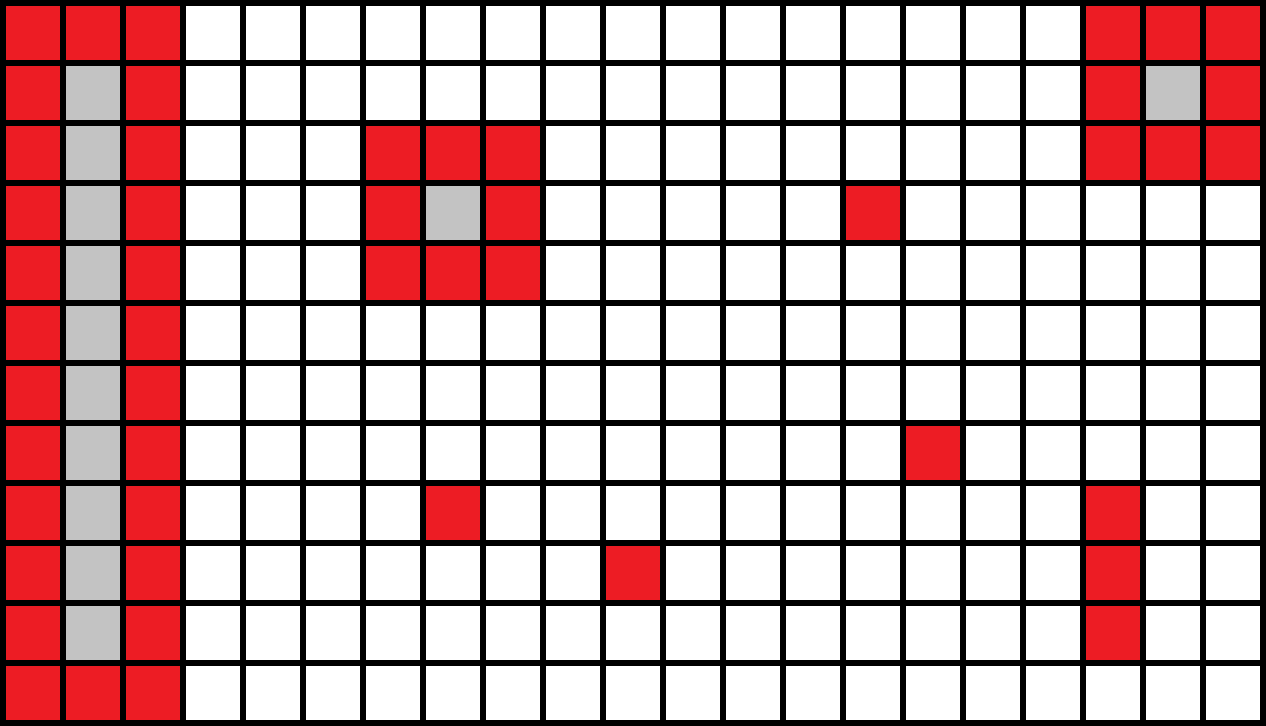
\includegraphics[width=170px]{otwarcie-morfologiczne-stan-po-erozji.png}}}
            \qquad
            \subfloat[\centering]{{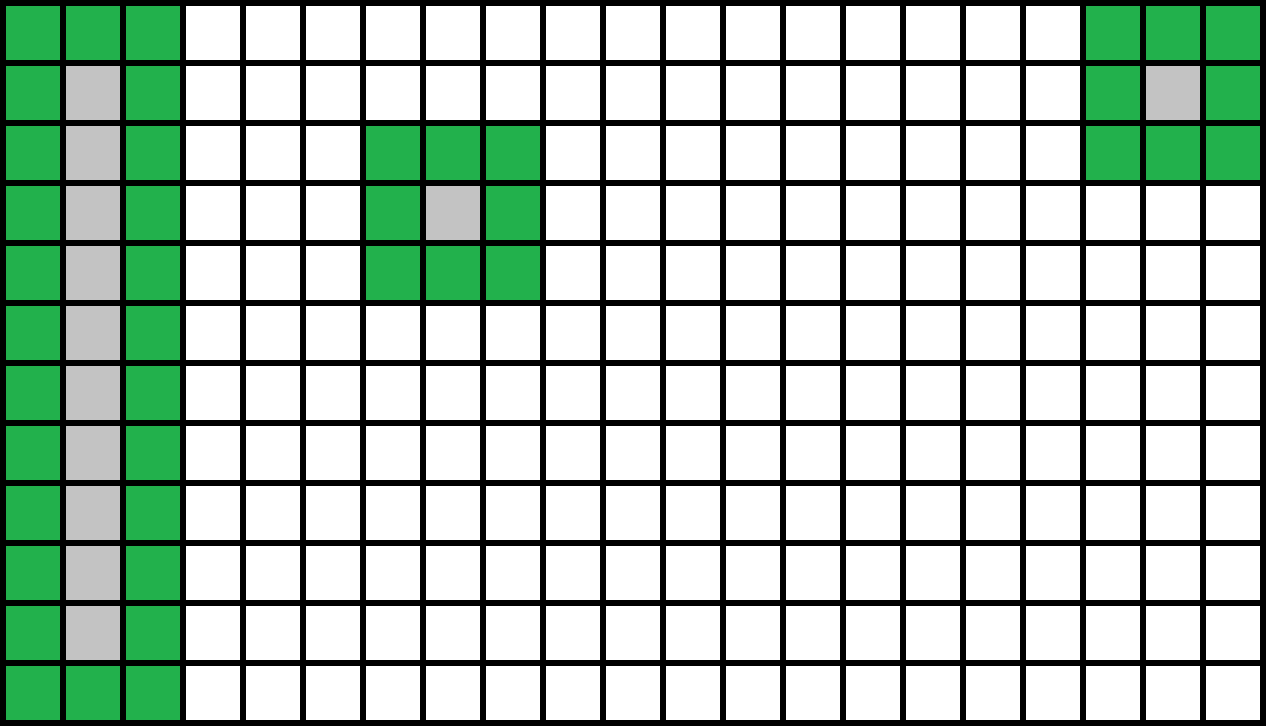
\includegraphics[width=170px]{otwarcie-morfologiczne-stan-po-dylatacji.png}}}
            \caption
            {
                (\textit{Opracowanie własne}) Otwarcie Morfologiczne.
                (a) Stan początkowy.
                (b) Stan po erozji z wykorzystaniem elementu strukturalnego z rysunku \ref{elementy_strukturalne}(a).
                (c) Stan po dylatacji z wykorzystaniem elementu strukturalnego z rysunku \ref{elementy_strukturalne}(a).
                Szarym kolorem zaznaczono piksele, które posiadają wartość 1, czerwonym te, które zmieniły wartość z 1 na 0. Zielonym natomiast zaznaczone te piksele, które zmieniły wartość z 0 na 1.
            }
            \label{Otwarcie_Morfologiczne}
        \end{figure}

        \subsection{Zamknięcie morfologiczne}
        {
            \label{sec:zamkniecie-morfologiczne}
            \Large
            \justifying
            \quad
            Zamknięcie morfologiczne - jest równoważne dwom następującym po sobie operacjom na obrazie: dylatacji, a następnie erozji.
            Wykonanie dylatacji, a następnie erozji pozwala na zamknięcie (przez zamknięcie należy rozumieć wypełnienie otworu wewnątrz obiektu, tak jak pokazano na Rysunku \ref{Zamkniecie_morfologiczne}(b)) niektórych obiektów, a następnie przywrócenie pozostałych obiektów do stanu sprzed dylatacji.
            Jak możemy zauważyć na Rysunku \ref{Zamkniecie_morfologiczne}(c), piskele, które wcześniej były odłączone od wiekszego obiektu ale leżały niedaleko teraz stanowią integralną jego cześć, a dwa większe obiekty połączyły się \cite{Digital Image Processing Second Edition}.
        }

        \begin{figure}[H]
            \centering
            \subfloat[\centering]{{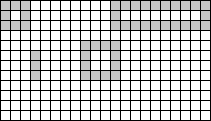
\includegraphics[width=170px]{zamkniecie-morfologiczne-stan-poczatkowy.png}}}
            \qquad
            \subfloat[\centering]{{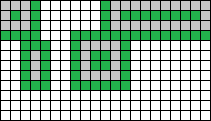
\includegraphics[width=170px]{zamkniecie-morfologiczne-stan-po-dylatacji.png}}}
            \qquad
            \subfloat[\centering]{{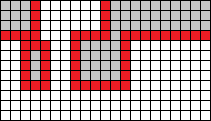
\includegraphics[width=170px]{zamkniecie-morfologiczne-stan-po-erozji.png}}}
            \caption
            {
                (\textit{Opracowanie własne}) Zamknięcie Morfologiczne.
                (a) Stan początkowy.
                (b) Stan po dylatacji z wykorzystaniem elementu strukturalnego z rysunku \ref{elementy_strukturalne}(a).
                (c) Stan po erozji z wykorzystaniem elementu strukturalnego z rysunku \ref{elementy_strukturalne}(a).
                Szarym kolorem zaznaczono piksele, które posiadają wartość 1, czerwonym te, które zmieniły wartość z 1 na 0. Zielonym natomiast zaznaczone te piksele, które zmieniły wartość z 0 na 1.
            }
            \label{Zamkniecie_morfologiczne}
        \end{figure}
        \subsection{Korekcja Gamma}
        {
            \label{sec:korekcja-gamma}
            \Large
            \justifying
            \quad
            Korekcja Gamma - operacja punktowa wykonywana na obrazie monochromatycznym, która bazuje na krzywej gamma i wyraża się ją za pomocą wzoru \(L'(x,y) = L(x,y)^\gamma\).
            Zastosowanie \(\gamma = 1\) sprawi, że obraz pozostanie bez zmian.
            Natomiast w przypadku, gdy \(\gamma > 1\) obraz zostanie przyciemniony.
            Analogicznie jest, gdy \(\gamma < 1\), to obraz zostanie rozjaśniony \cite{Digital Image Processing Second Edition}.
        }
        \begin{figure}[H]
            \centering
            \subfloat[\centering]{{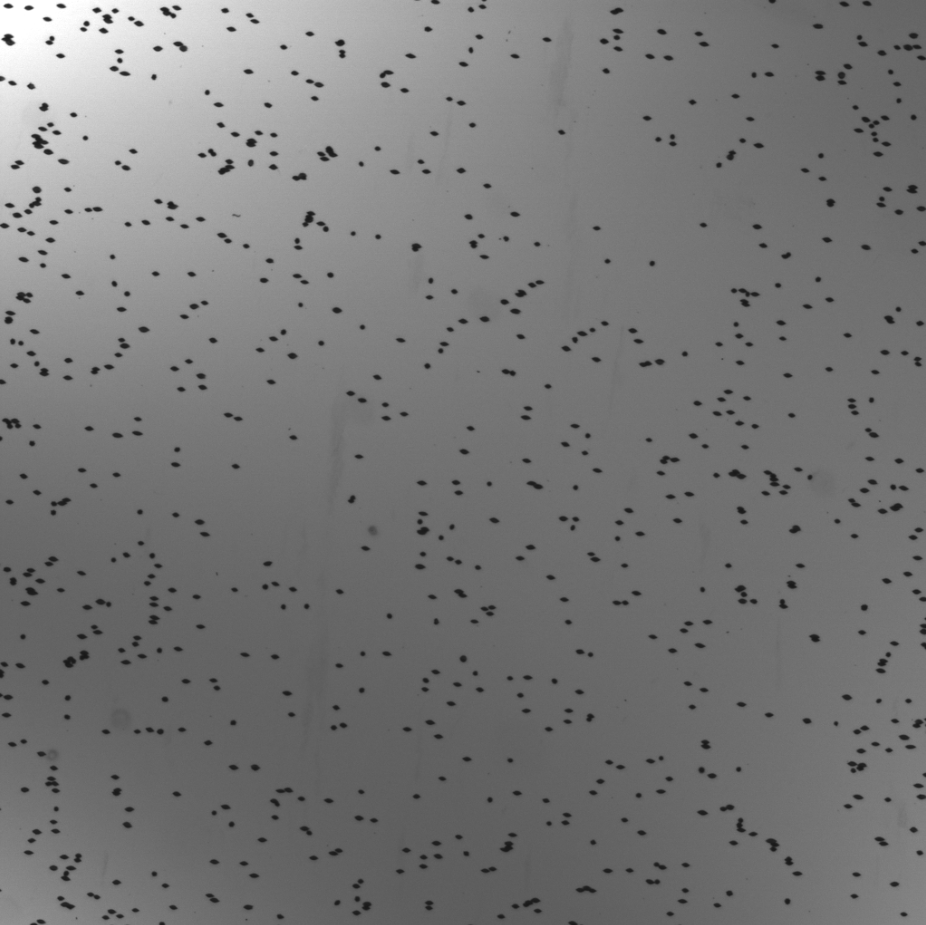
\includegraphics[width=170px]{GammaCorrection_Start.png}}}
            \qquad
            \subfloat[\centering]{{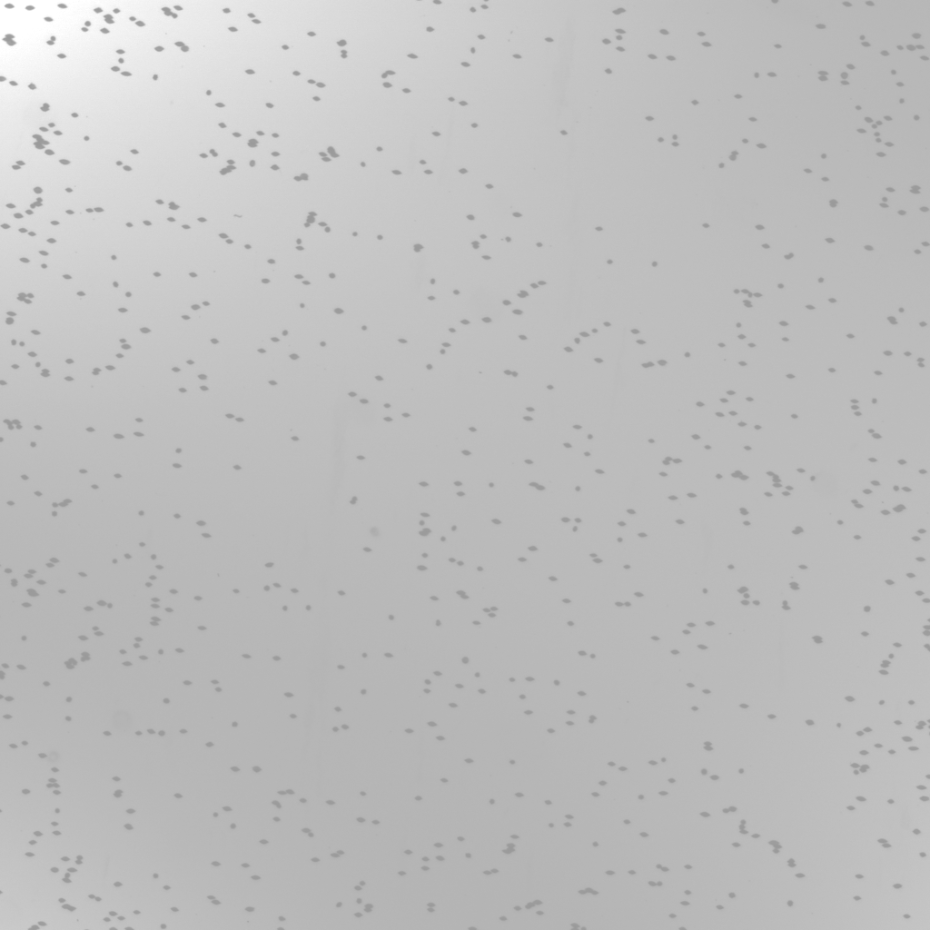
\includegraphics[width=170px]{GammaCorrection_Rozjasnienie085.png}}}
            \qquad
            \subfloat[\centering]{{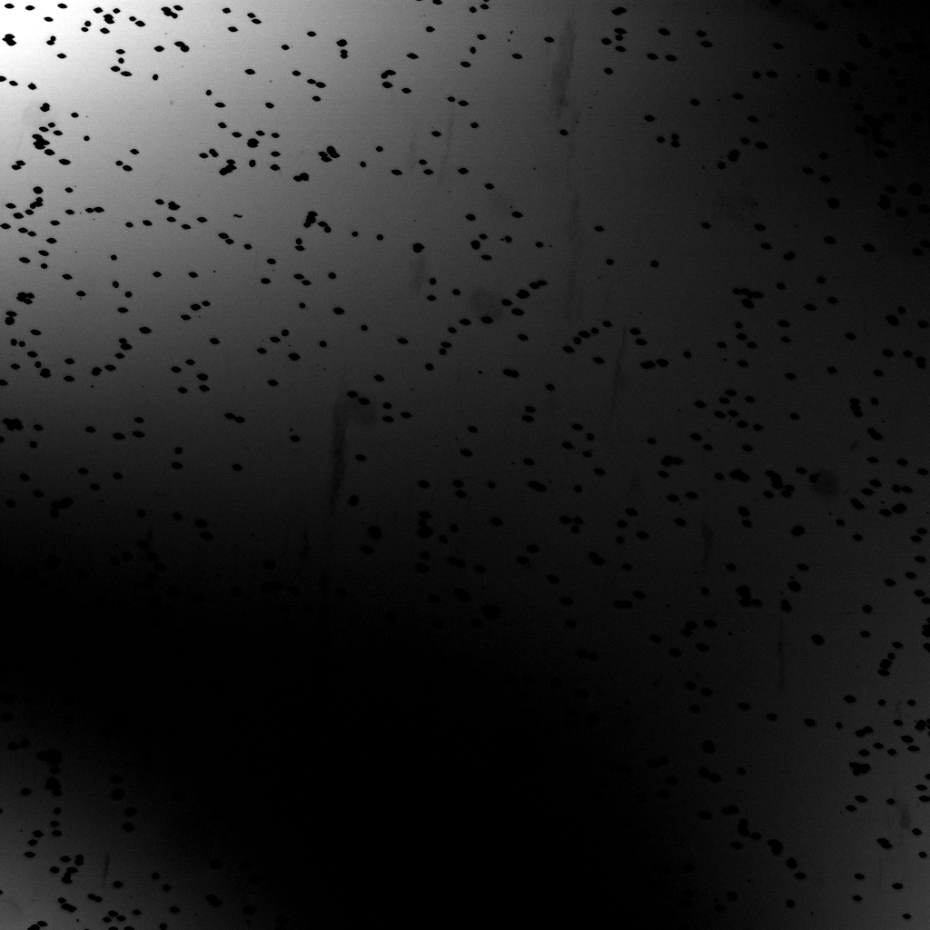
\includegraphics[width=170px]{GammaCorrection_Przyciemnienie110.png}}}
            \caption
            {
                (\textit{Opracowanie własne}) Korekcja Gamma.
                (a) Stan początkowy.
                (b) Stan po korekcji gamma z parametrem \textit{0.85}.
                (c) Stan po korekcji gamma z parametrem \textit{1.10}.
            }
            \label{Korekcja_Gamma}
        \end{figure}
    \section{Część Praktyczna}

        \subsection{Wykorzystane oprogramowanie}
        \subsubsection{Gimp 2.10.22}
        {
            \label{sec:gimp}
            \Large
            \justifying
            \quad
            Gimp 2.10.22 - program graficzny służący do tworzenia i edycji grafiki rastrowej \cite{Program GIMP}.
            Program został wykorzystany do przygotowania wszystkich grafik znajdujących się w pracy oznaczonych słowami \emph{``opracowanie własne''}.
        }

        \subsubsection{CMake 3.19.0}
        {
            \label{sec:cmake}
            \Large
            \justifying
            \quad
            CMake 3.19.0 - oprogramowanie, które służy do testowania, budowania oraz upakowania źródeł programu.
            CMake został wykorzystany do wygenerowania projektów na podstawie źródel biblioteki \emph{LibTIFF}.
            Wyżej wymienione projekty mogą można otworzyć, a następnie zbudować za pomocą programu {Visual Studio 2019} \cite{Program CMake}.
        }

        \subsubsection{LibTIFF 4.2.0}
        {
            \label{sec:LibTIFF}
            \Large
            \justifying
            \quad
            LibTIFF 4.2.0 - biblioteka służąca do manipulacji obrazami typu TIFF, typ ten dokładniej został opisany w rozdziale \ref{sec:rozszerzenie-tiff}.
            Biblioteka została wybrana, ponieważ pozwala w łatwy sposób odczytywać informacje zapisane w obrazach.
            Napisana jest w języku C, więc w łatwy sposób można wykorzystać ją w programach pisanych w języku C++ \cite{Biblioteka LibTIFF}.
        }
        \subsubsection{Visual Studio 2019}
        {
            \label{sec:VisualStudio2019}
            \Large
            \justifying
            \quad
            Visual Studio 2019 - doskonały program do pisania oprogramowania wykorzystując technologie pochodzące od firmy \emph{Microsoft} \cite{VS2019}.
            W Visual Studio 2019 jak nigdzie indziej można z powodzeniem łączyć języki C++ oraz C\# za pomocą C++/CLI.
            Dzięki takim możliwościom, można z powodzeniem tworzyć oprogramowanie składające się z wielu mniejszych programów, które napisane są w różnych językach.
            Dla przykładu: tworzymy bibliotekę napisaną w C++, ponieważ zależy nam na tym, aby operacje wykonywały się bardzo szybko.
            Interfejs użytkownika jest napisany w C\#, ponieważ robi się to w prosty i szybki sposób.
            Następnie całość łączymy wykorzystując C++/CLI.
            Wynikiem takiego działania będzie program posiadający interfejs graficzny i łączący w sobie C++ oraz C\#.
        }
        \subsubsection{\LaTeX}
        {
            \label{sec:LaTeX}
            \Large
            \justifying
            \LaTeX - wysokiej jakości system służący do tworzenia dokumentów w przystępny sposób \cite{LaTeX}.
            Dzięki \LaTeX, proces tworzenia spisu treści, spisu grafik czy bibliografii jest automatyzowany.
            Odwołania do konkretnych rozdziałów, podrozdziałów czy źródeł to kwestia wywołania funkcji \emph{cite} lub \emph{ref}.
            Jest standardem publikacji dokumentów naukowych i technicznych.
        }
        \subsubsection{Visual Studio Code}
        {
            \label{sec:VisualStudioCode}
            \Large
            \justifying
            \quad
            Visual Studio Code - uniwersalny edytor z ogromną bazą rozszerzeń, dostępny na każdej z platform \emph{Windows}, \emph{Linux} oraz \emph{MacOS}, umożliwiający tworzenie oprogramowania niemal w każdym języku \cite{VSCode}.
            W swojej pracy wykorzystałem \emph{Visual Studio Code} jako edytor tekstowy plików z rozszerzeniem \emph{tex}, które następnie były wykorzystywane przez program \LaTeX (\ref{sec:LaTeX}).
        }
        \subsubsection{.NET Framework 4.7.2}
        {
            \label{sec:.NETFramework 4.7.2}
            \Large
            \justifying
            \quad
            .NET Framework 4.7.2 - oprogramowanie stworznone przez firme \textit{Mircosoft} pozwalające na
            tworzenie szerokiej gamy aplikacji, które działają głownie na systemach \textit{Windows}.
            W kontekscie tej pracy .NET Framework 4.7.2 został wykorzystany w celu uruchomienia zarówno kodu zarządzalnego (napisanego w języku C\#)
            oraz natywnego (napisanego w języku C++) \cite{.NET Framework}.
        }
        \subsubsection{nlohmann.json 3.9.1}
        {
            \label{sec:nlohman.json 3.9.1}
            \Large
            \justifying
            \quad
            nlohmann.json 3.9.1 - prosta w obsłudze biblioteka pozwalająca na tworzenie, modyfikowanie oraz odczytywanie informacji
            z obiektów typu \textit{json} \cite{nlohmann.json 3.9.1}.
        }
        \subsubsection{OpenMP 5.1}
        {
            \label{sec:openmp}
            {
                \Large
                \justifying
                \quad
                \color{blue}
                {
                OpenMP 5.1 - oprogramowanie slużące do programowania równoległego \cite{OpenMP 5.1}.
                W bibliotece, o której traktuje ta praca, \emph{OpenMP 5.1} zostało wielokrotnie wykorzystane do zrównoleglania pętli \emph{for}.
                Dzięki temu niektóre operacje wykonują się kilka razy szybciej.
                }
            }
        }
        \subsection{Budowa oprogramowania}
        {
            \Large
            \justifying
            \quad
            Aby wykorzystac bibliotekę BIA.Core w swoim projekcie, należy najpierw zbudować tę bibliotekę.
            Kolejnym etapem jest wykorzystanie plików zawartych w katalogu, do którego biblioteka zostanie zbudowana,
            oraz dodanie pliku ``BIA.h'' za pomocą dyrektywy \textit{\#include}.
            Wykorzystanie biblioteki LibTIFF 4.2.0 w programie pisanym w języku C++ opartym o MSBuild polega na tym, że należy najpierw ręcznie zbudować tę bibliotekę przy użyciu narzędzia \textit{nmake} oraz \textit{Command Prompt for Visual Studio 2019} \cite{Biblioteka LibTIFF}.
            W związku z powyższym, w programie \textit{Visual Studio 2019} trzeba dodać ścieżkę do miejsca, w którym znajduje się zbudowana przez nas biblioteka.
            Przykładowo ``D:/tiff-4.2.0/libtiff''.
        }
        \subsection{Diagramy klas}
        \begin{figure}[H]
            \centering
            \subfloat[\centering]{{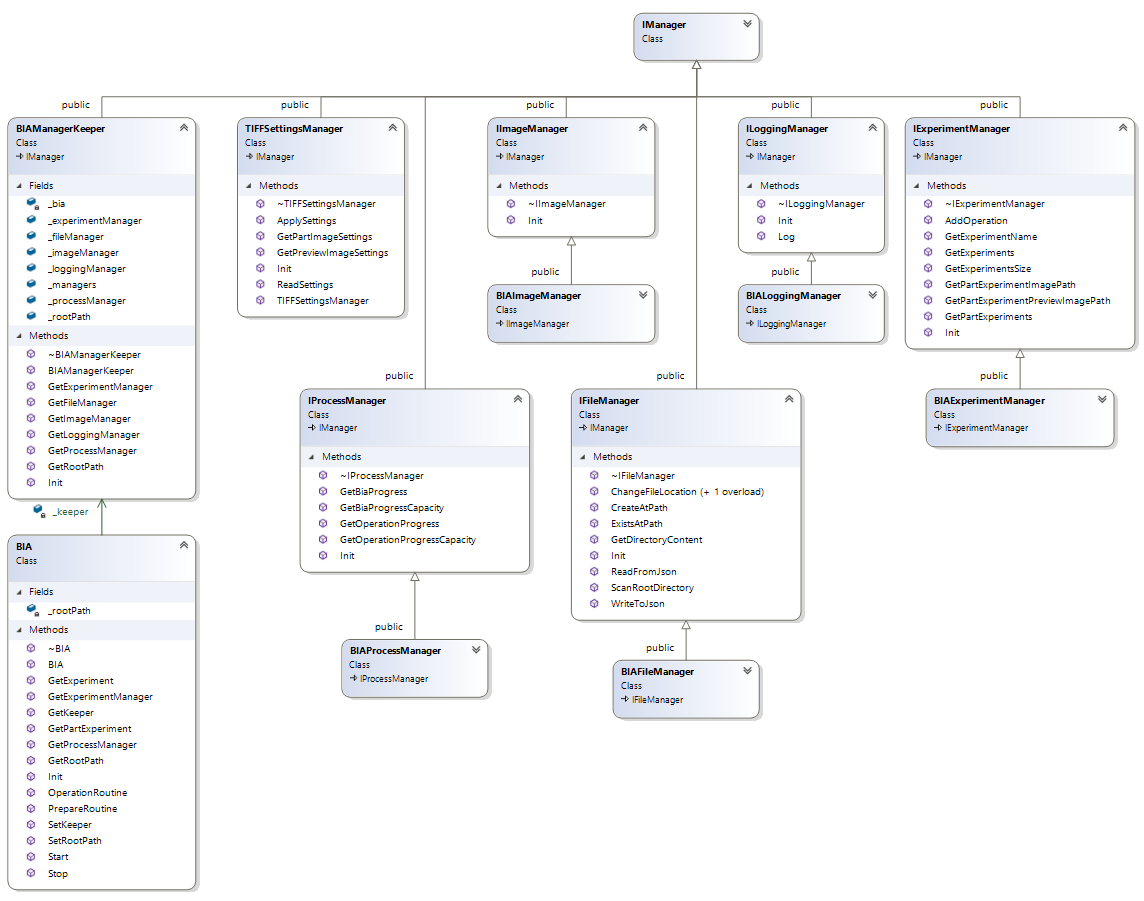
\includegraphics[width=\textwidth]{MainClassDiagram.png}}}
            \qquad
            \subfloat[\centering]{{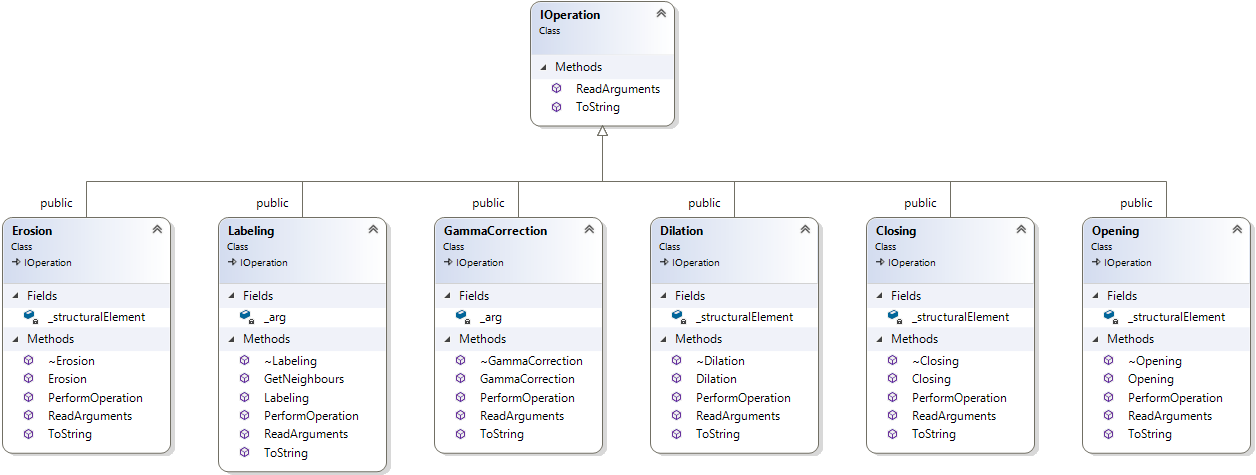
\includegraphics[width=\textwidth]{OperationClassDiagram.png}}}
            \caption
            {
                (\textit{Opracowanie własne}) Diagramy klas biblioteki BIA.Core.\\
                (a) Główny diagram klas. Przedstawione na nim klasy odpowiadają za najwazniejsze funkcje biblioteki.\\
                (b) Diagram klas przedstawiający operacje, których wykonanie na obrazach umożliwia biblioteka.
            }
            \label{class_diagram}
        \end{figure}
        \subsection{Omówienie implementacji}
        {
            \label{omowienieimplementacji}
            \Large
            \justifying
            \quad
            Biblioteka, która opisywana jest w tej pracy nosi nazwę ``BIA.Core''.
            Całe rozwiązanie składa się jeszcze z dwóch innych projektów: ``BIA.UI'' oraz ``BIA.Bridge''.
            ``BIA.UI'' to biblioteka napisana w języku C\#, stanowiąca interfejs użytkownika. Służy do pokazania funkcjonalności biblioteki ``BIA.Core''.
            Wspomniany wcześniej projekt ``BIA.Bridge'' stanowi połączenie (\emph{bridge} z ang. \emph{most}) między interfejsem użytkownika, a biblioteką ``BIA.Core''.
            Główną klasą biblioteki ``BIA.Core'' jest klasa ``BIA'' (Rysunek \ref{class_diagram} podpunkt (a)).
            Nazwa jej pochodzi od angielskich słów ``Blood Image Analyzer'', czyli ``Analizator Obrazów Krwi''.
            Głównym zadaniem klasy ``BIA'' jest zebranie wszystkich funkcjonalności biblioteki w wygodny do użycia sposób.
            Zawiera ona prywatne pole o nazwie ``\_rootPath'', które jest odpowiedzialne za przetrzymywanie ścieżki do wybranego przez nas katalogu.
            W bibliotece ``BIA.Core'' nazwy wszystkich interfejsów zaczynają się od litery ``I''. 
            ``BIA'' posiada wskaźnik typu ``BIAManagerKeeper'', który zawiera w sobie klasy implementujące odpowiednie interfejsy.
            Jest odpowiedzialny za ich inicjalizację oraz późniejsze wykorzystanie.
            Każdy z interfejsów niesie ze sobą funkcjonalności w zależnosci od nazwy: 
            ``IImageManager'' - zarządzanie obrazami, ``IExperimentManager'' - zarządzanie eksperymentami,
            ``IFileManager'' - zarządzanie plikami, ``IProcessManager'' - zarządzanie asynchronicznymi procesami,
            ``ILoggingManager'' - logowanie do pliku.
            Każdy z menadżerów implementuje odpowiedni interfejs:
            ``BIAImageManager'' implementuje ``IImageManager'',
            ``BIAExperimentManager'' implementuje ``IExperimentManager'',
            ``BIAFileManager'' implementuje ``IFileManager'',
            ``BIAProcessManager'' implementuje ``IProcessManager'',
            ``BIALoggingManager'' implementuje ``ILoggingManager''.
            Klasa ``BIA'' pozwala na wykorzystanie niektórych funkcjonalnosci menadżerów poza biblioteką ``BIA.Core''.
            Służą do tego funkcje: ``GetExperimentManager'', która zwraca wskaźnik typu ``IExperimentManager'',
            ``GetProcessManager'', która zwraca wskaźnik typu ``IProcessManager''.
            Z punktu widzenia użytkownika biblioteki wykorzystanie pozostałych menadżerów nie jest konieczne, ponieważ wykonują swoje operacje automatycznie - w zależności od kontekstu.
            Aby poprawnie skorzystać z funkcjonalności klasy ``BIA'' należy po stworzeniu obiektu tej klasy wywołać funkcję ``Init''.
            Funkcja ta odpowiedzialna jest za utworzenie wszystkich potrzebnych obiektów, w tym inicjalizacje ``BIAManagerKeeper''.
            Gdy ``BIAManagerKeeper'' zostanie zainicjalizowany, utworzeni zostają pozostali menadżerowie.
            Domyślny konstruktor klasy ``BIA'' przyjmuje jako parametr ścieżkę do katalogu, która następnie zostaje zapisana do zmiennej ``\_rootPath''.
            Jest to bardzo ważna rzecz, gdyż od tego zależy poprawne funkcjonowanie całej biblioteki.
            Destruktor ``$\sim$BIA'' działa w taki sposób, że gdy zostanie wywołany to usunięte zostają wszystkie obiekty, któych używa biblioteka.
            Zapobiega to wyciekaniu pamięci, a także jej niekontrolowanemu wykorzystaniu.
            Funkcja ``GetKeeper'' zwraca wskaźnik do obiektu ``BIAManagerKeeper''.
            ``GetRootPath'' pozwala na otrzymanie ścieżki, do głównego katalogu.
            ``OperationRoutine'' wykonuje operacje (operacje zapisywane są w pliku 
            ``recipe.json'') na każdym z obrazów.
            ``PrepareRoutine'' dzieli główne obrazy na mniejsze i przygotowuje wszystkie potrzebne do późniejszej fazy pliki.
            Obydwie powyższe metody można uruchomić w sposób asynchroniczny za pomocą ``BIAProcessManager'', nie jest to jednak przymus.
            ``SetKeeper'' pozwala na ustawienie obiektu ``BIAManagerKeeper''.
            ``SetRootPath'' pozwala na zmiane ścieżki do katalogu głównego.
            ``Start'' odpowiada za uruchomienie odpowiedniego procesu. Jako argument przyjmuje typ wyliczeniowy o nazwie ``EProcess'', jeżeli ustalimy jego wartość na ``EProcess::BIAPROCESS'' to ``BIAProcessManager'' uruchomi asynchronicznie funkcje ``PrepareRoutine''.
            W przypadku wartosci ``EProcess::BIAOPERATIONS'' uruchomiona zostanie funkcja ``OperationRoutine'', również w sposób asynchroniczny.
            Funckja ``OperationsRoutine'' wykonuje operacje zapisane w pliku ``recipe.json'' dla każdego obrazu.
            Funckja ``Stop'' pozwala na zatrzymanie operacji niezależnie od tego, którą z nich uruchomiliśmy wcześniej.
            Zatrzymanie procesów pozwala na oszczędzenie sporej ilości czasu w przypadku, gdy przewidujemy, że proces nie przyniesie pożądanych efektów i chcemy nanieść korekty.
            Zapisana do zmiennej ``\_rootPath'' ścieżka będzie postrzegana jako źródło tak zwanych ``eksperymentów''.
            Przez ``eksperyment'' należy rozumieć katalog, w którym znajdują się dwa zdjęcia pochodzące z mikroskopu.
            Zdjęcia te powinny wcześniej zostać wyeksportowane do plików o typie ``.tif'' oraz nazwane w odpowiedni sposób.
            Zdjęcie zorientowane horyzontalnie powinno zawierać w swojej naziwe słowo ``horizontal'', natomiast te zorientowane wertykalnie - ``vertical''.
            Dzięki temu obrazy zostaną zlokalizowane, odpowiednie nazwnictwo pozwoli na zastosowanie odpowiednich ustawień do danego ułożenia obrazu.
            Wewnątrz eksperymentu utworzone zostaną dwa katalogi: ``Horizontal'' oraz ``Vertical''.
            W kolejnym kroku utworzone zostaje po czterdzieści katalogów wewnątrz każdego z podkatalogów eksperymentu.
            Do każdego z tych podkatalogów trafia fragment obrazu głównego, który będzie podlegał różnym operacjom.
            Na potrzeby biblioteki, dla każdego z wydzielonych obrazów utworzone zostają też pliki: ``preview.tif'', ``recipe.json'' oraz ``results.json''.
            Plik ``preview.tif'' to zbinaryzowany obraz wynikowy, ``recipe.json'' zawiera spis operacji, które mają zostać wykonane na obrazie binarnym, ``results.json'' to plik, do którego zapisywane są wyniki operacji etykietowania (ang \emph{labeling}).
            Etykietowanie to operacja, która pozwala na zliczanie obiektów znajdujących się na obrazie binarnym w zależności od tego jaką wartość przyjmujemy jako tło.
            W przypadku tej biblioteki tło jest zaznaczane białym kolorem.
            Kod źródłowy z racji swojej znaczącej objętości został umieszczony jako załącznik do tej pracy.
            Wszystkie algorytmy są autorskie.
            }
            \newline\newline
            {
                \label{iprocessmanager}
                \Large
                \justifying
                \quad
                IProcessManager - zaimplementowany przez klase ``BIAProcessManager'' pozwala na śledzenie postępu wykonywanych operacji.
                Opis funkcji: ``GetBiaProgress'' pozwala na otrzymanie aktualnego postępu w przygotowywaniu głównego katalogu.
                ``GetBiaProgressCapacity'' zwraca całkowitą ilość operacji przygotowywania katalogu głownego.
                ``GetOperationProgress'' zwraca aktualny postęp procesu przetwarzania obrazów.
                ``GetOperationProgressCapacity'' zwraca całkowitą ilośc operacji przetwarzania obrazów.
            }
            \newline\newline
            {
                \label{iexperimentmanager}
                \Large
                \justifying
                \quad
                IExperimentManager - zaimplementowany przez klase ``BIAExperimentManager'' pozwala na wykonywanie pewnych funkcji na eksperymentach.
                Opis funkcji: ``AddOperation'' pozwala na dodanie operacji do danego eksperymentu częściowego.
                ``GetExperimentName'' zwraca nazwe eksperymentu na podstawie identyfikatora.
                ``GetExperiments'' zwraca wszystkie istniejące eksperymenty.
                ``GetExperimentsSize'' zwraca ilość eksperymentów.
                ``GetPartExperimentImagePath'' zwraca ścieżkę do danego obrazu na podstawie nazwy eksperymentu, identyfikatora eksperymentu częsciowego oraz tego, czy obraz ten należy do folder ``Vertical'' czy ``Horizontal''.
                ``GetPartExperimentPreviewImagePath'' podobnie jak w przypadku poprzedniej funkcji na podstawie takich samych argumentów zwraca ścieżkę do obrazu wyjściowego (powstałego po podzieleniu obrazu głównego).
                ``GetPartExperiments'' zwraca eksperymenty częściowe na podstawie identyfikatora eksperymentu oraz przynależności do folder ``Vertical'' lub ``Horizontal''.
            }
        \begin{figure}[H]
            \centering
            \subfloat[\centering]{{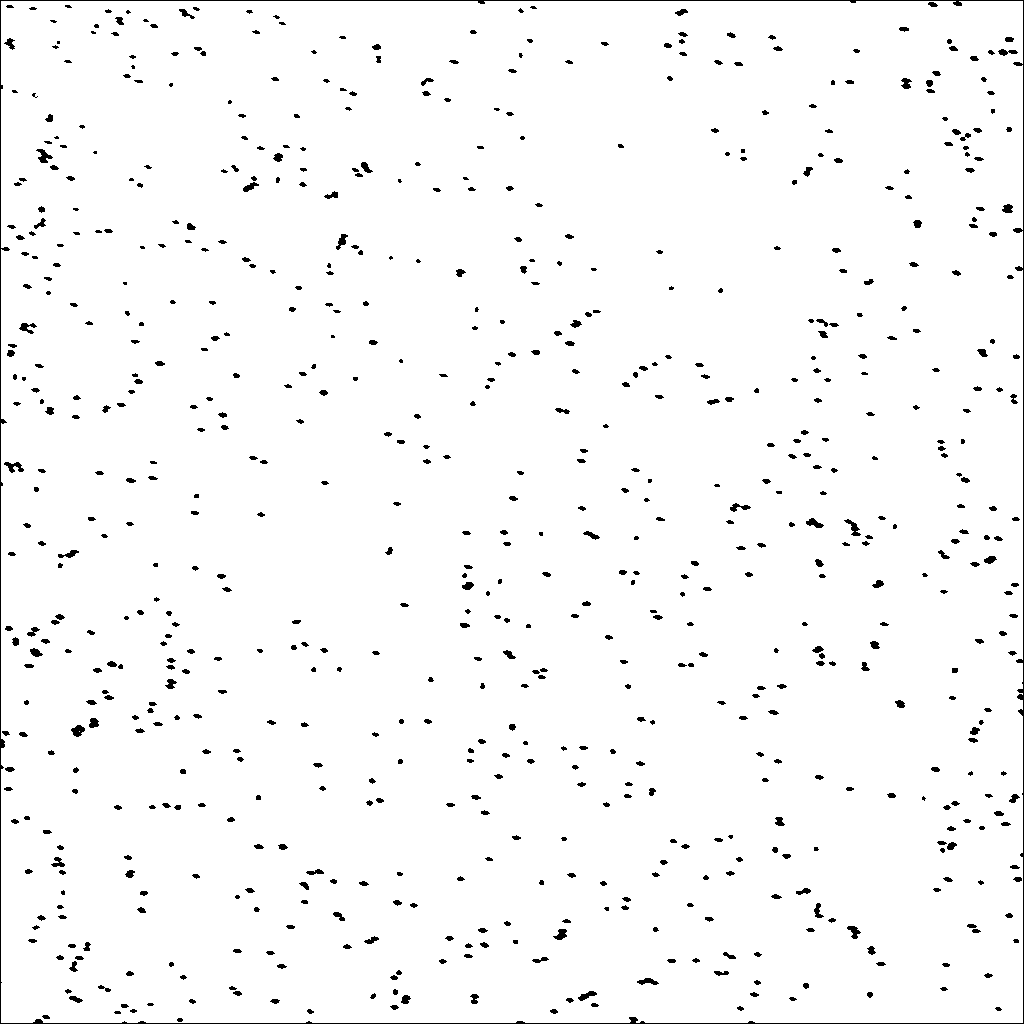
\includegraphics[width=170px, height=170px]{preview.png}}}
            \qquad
            \subfloat[\centering]{{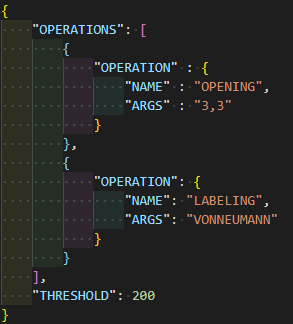
\includegraphics[height=170px, width=170px]{recipejson.png}}}
            \qquad
            \subfloat[\centering]{{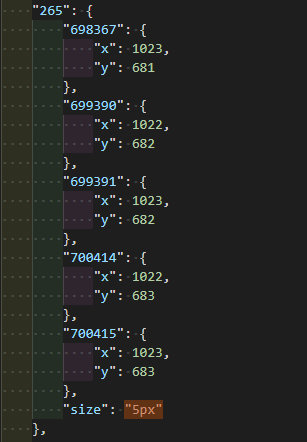
\includegraphics[height=220px]{resultsjson-wholeobj.png}}}
            \qquad
            \subfloat[\centering]{{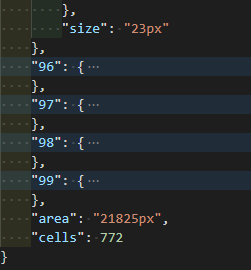
\includegraphics[height=170px]{resultsjson-ending.png}}}
            \caption
            {
                (\textit{Opracowanie własne}) Przykłady plików.\\
                (a) Zbinaryzowany obraz wynikowy.\\
                (b) Przykład pliku ``recipe.json''. Tablica ``OPERATIONS'' zawiera liste operacji, które mają zostać wykonane na danym obrazie.
                    W tym przypadku zostaną wykonane dwie operacje: Otwarcie morfologiczne (rozdział \ref{sec:otwarcie-morfologiczne}) elemntem strukturalnym o rozmiarach 3 na 3.
                    Drugą operacją jest etykietowanie wykorzystując sąsiedztwo Vonneumann'a (rozdział \ref{sec:sasiedztwo}).
                    Zapisana w polu ``THRESHOLD'' wartość stanowi argument operacji binaryzacji.\\
                (c) Przykład pliku ``results.json''. Na rysunku przedstawiony jest obiekt, któremu nadano etykietę ``265''.
                    Piksele, z których dany obiekt się zkłada mają odpowiednio indeksy ``698367'', ``699390'', ``699391'', ``700414'', ``700415''.
                    Każdy z nich posiada współrzędne zapisane w polach ``x'' oraz ``y''.
                    Pole ``size'' zawiera informacje o tym jaki rozmiar ma dany obiekt.\\
                (d) Przykład zakończenia pliku ``results.json''. Pole ``area'' zawiera sume powierzchni obiektów znalezionych na obrazie,
                    Natomiast pole ``cells'' to liczba znalezionych obiektów 
                    (obiekty o etykietach ``96'', ``97'', ``98'', ``99'' mogą sugerować, że obiektów jest tylko 99 pomimo wartości ``cells'' 772. Należy jednak pamiętać o tym, że obiekty są zapisywane do pliku w kolejności losowej).
                \label{przykladowepliki}
            }
        \end{figure}
        \subsection{Omówienie interfejsu aplikacji okienkowej}
        {
            \label{iexperimentmanager}
            \Large
            \justifying
            \begin{figure}[H]
                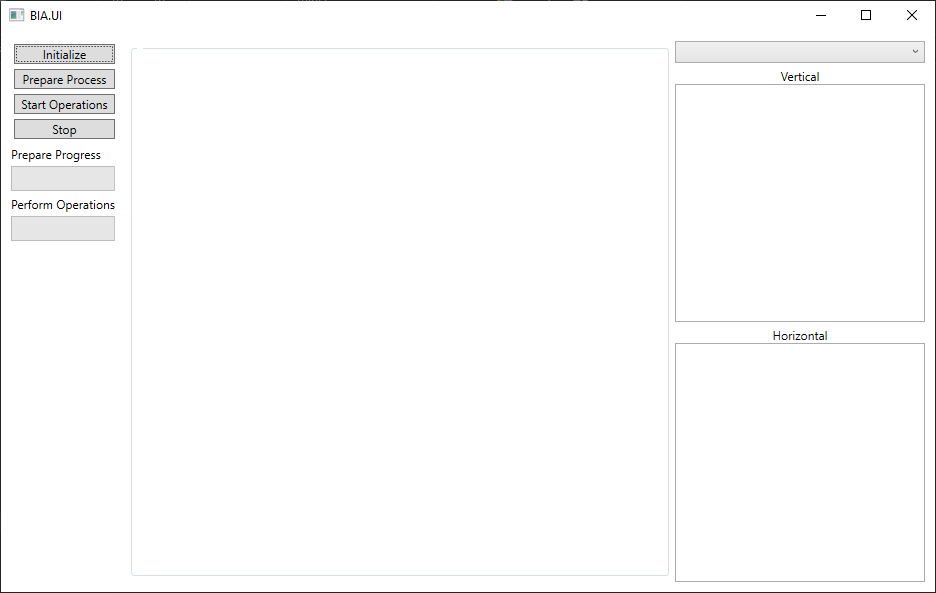
\includegraphics[width=\textwidth]{okienkowa-start.png}
                \caption{(Opracowanie własne) Widok aplikacji okienkowej tuż po jej uruchomieniu.}
                \label{okienkowaapkastart}
            \end{figure}
            \begin{figure}[H]
                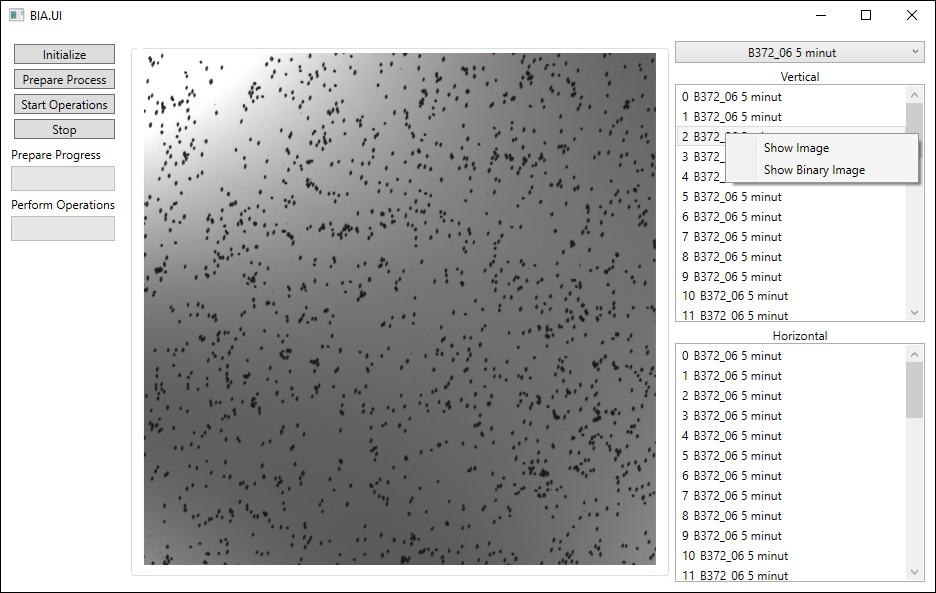
\includegraphics[width=\textwidth]{context-menu.png}
                \caption{(Opracowanie własne) Widok aplikacji okienkowej po kliknięciu przycisku ``Initialize'' oraz wybraniu eksperymentu ``B372\_06 5 minut'' oraz kliknięciu prawym przyciskiem myszy na jeden z eksperymentów częściowych.}
                \label{okienkowaapkacontextmenu}
            \end{figure}
            \begin{figure}[H]
                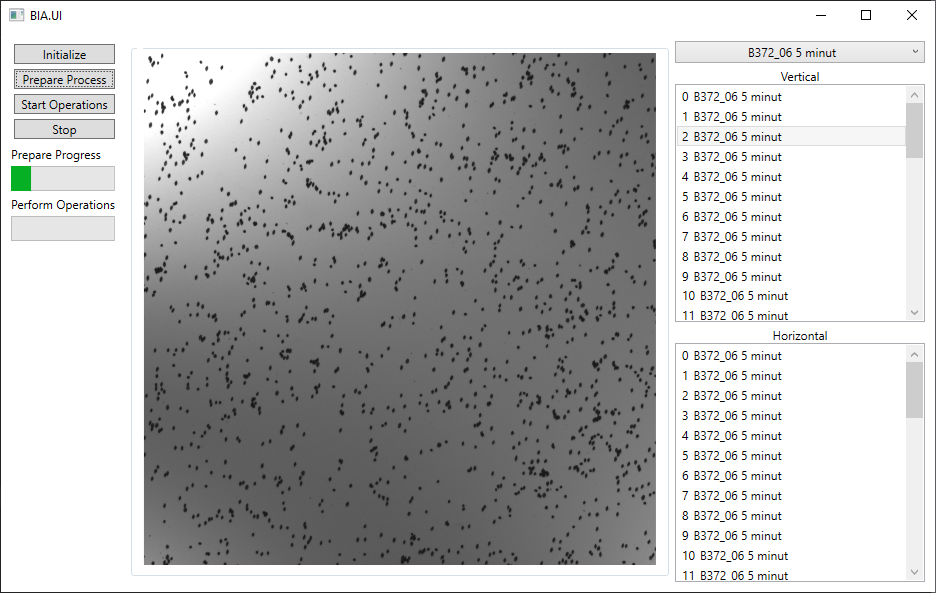
\includegraphics[width=\textwidth]{okienkowa-biaa.png}
                \caption{(Opracowanie własne) Widok aplikacji okienkowej po kliknięciu przycisku ``Prepare Process''.
                Poniżej napisu ``Prepare Process'' można obserwować postęp tego procesu.}
                \label{okienkowaapkabiaa}
            \end{figure}
            \begin{figure}[H]
                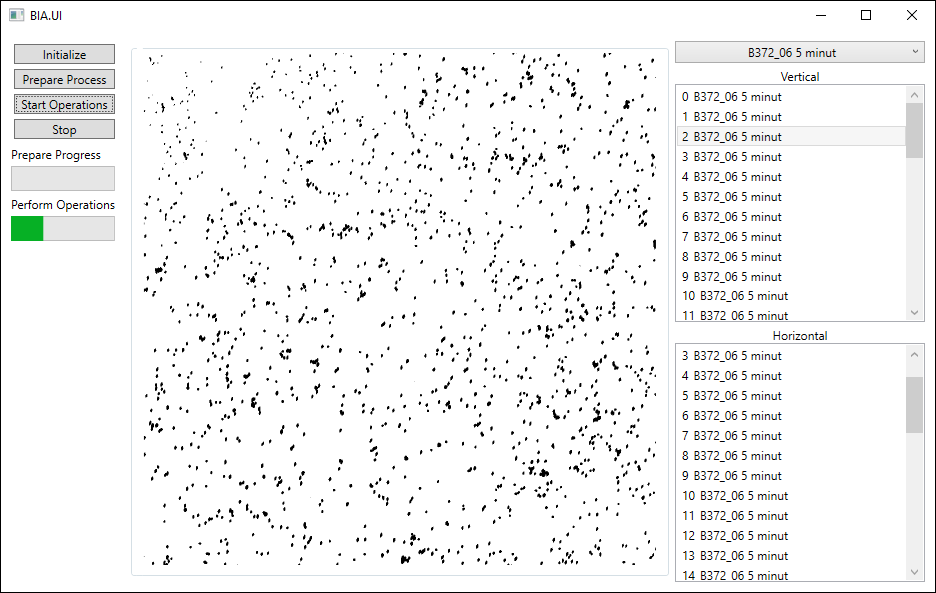
\includegraphics[width=\textwidth]{okienkowa-oper.png}
                \caption{(Opracowanie własne) Widok aplikacji okienkowej po kliknięciu przycisku ``Start Operations''.
                Poniżej napisu ``Perform Operations'' można obserwować postęp tego procesu.}
                \label{okienkowaapkaoper}
            \end{figure}
            \label{implementacjaokienko}
            \Large
            \justifying
            \quad
            Jak można zauważyć na rysunkach \ref{okienkowaapkastart}, \ref{okienkowaapkacontextmenu}, \ref{okienkowaapkabiaa} oraz \ref{okienkowaapkaoper}
            aplikacja okienkowa składa się z kilku elementów.
            Cztery przyciski po lewej stronie odpowiadają za: ``Initialize'' inicjalizacje obiektu klasy ``BIA'' pochodzącej z biblioteki ``Bia.Core'',
            ``Perpare Process'' uruchamia asynchronicznie proces przygotowania katalogu głównego.
            ``Start Operations'' uruchamia asynchronicznie proces przetwarzania obrazów,
            ``Stop'' umożliwia zatrzymanie wyżej wymienionych procesów.
            Dwa paski postępu poniżej informują nas o postępie wykonania odpowiedniego procesu.
            Na rysunku \ref{okienkowaapkabiaa} widać postęp w wykonaniu procesu ``Prepare Process'', z kolei na rysunku \ref{okienkowaapkaoper} postęp wykonania procesu przetwarzania obrazów.
            Środek okna zajmuje kontrolka służąca do wyświetlania obrazów. Obraz ładowany jest w momencie gdy wybierzemy za pomocą menu kontekstowego opcje ``Show Image'' lub ``Show Binary Image'' tak jak na rysunku \ref{okienkowaapkacontextmenu}.
            Po prawej stronie aplikacji znajduje się kontrolka o nazwie ``ComboBox'', która służy do wyboru danego eksperymentu za pomocą jego nazwy.
            Poniżej można znaleźć dwie kontrolki o nazwie ``ListBox'', które służą do wyświetlania list elementów.
            W kontekscie tej aplikacji wyświetlane są eksperymenty częściowe, które należą do wybranego wcześniej eksperymentu.
        }
    \newpage
    \section{Wyniki i dyskusja}
    \subsection{Przygotowanie katalogu głównego}
    \begin{figure}[H]
        \centering
        \subfloat[\centering]{{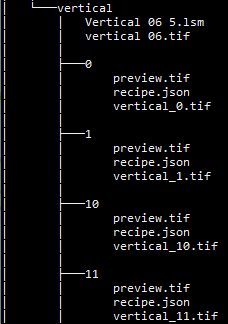
\includegraphics[height=220px]{poczatkowetreevertical.png}}}
        \qquad
        \subfloat[\centering]{{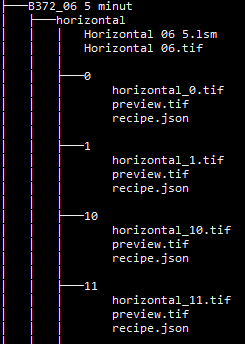
\includegraphics[height=220px]{poczatkowetreehorizontal.png}}}
        \qquad
        \subfloat[\centering]{{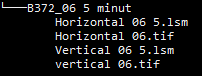
\includegraphics{poczatkowetree.png}}}
        \caption
        {
            (\textit{Opracowanie własne}) Przykłady przygotowania katalogu głównego.\\
            (a) Folder ``vertical'' po przeprowadzeniu procesu przygotowania katalogu głównego.\\
            (b) Folder ``horizontal'' po przeprowadzeniu procesu przygotowania katalogu głównego.\\
            (c) Folder główny przed uruchomienie procesu przygotowania katalogu głównego.\\
        }
        \label{przygotowanie katalogu glownego}
    \end{figure}
    {
        \label{przygotowaniekataloguglownego}
        \Large
        \justifying
        \quad
        Na rysunku \ref{przygotowanie katalogu glownego} możemy zauważyć jak wygląda drzewo folderów po przeprowadzeniu procesu przygotowania katalogu głownego.
        Nazwa eksperymentu to ``B372\_06 5 minut'' co możemy zauważyć na rysunku \ref{przygotowanie katalogu glownego} (b).
        W tym eksperymencie zostały stworzone dwa foldery ``vertical'' oraz ``horizontal''.
        W każdym z tych folderów znajduje się czterdzieści eksperymentów cześciowych noszących nazwy od 0 do 39.
        Każdy z eksperymentów częściowych posiada pliki ``preview.tif'', ``recipe.json'' oraz obraz wynikowy (powstały z podzielenia obrazu głównego).
        W ramach eksperymentu wyróżniamy dwa obrazy główne, w tym przypadku - ``Vertical 06.tif'' oraz ``Horizontal 06.tif''.
        Powstają z nich obrazy wynikowe, które trafiają do poszczególnych eksperymentów częsciowych.
        Ich przykładowe nazwy to ``vertical\_0.tif'' czy ``horizontal\_0.tif''.
    }
    \subsection{Przykład Binaryzacji}
    \begin{figure}[H]
        \centering
        \subfloat[\centering]{{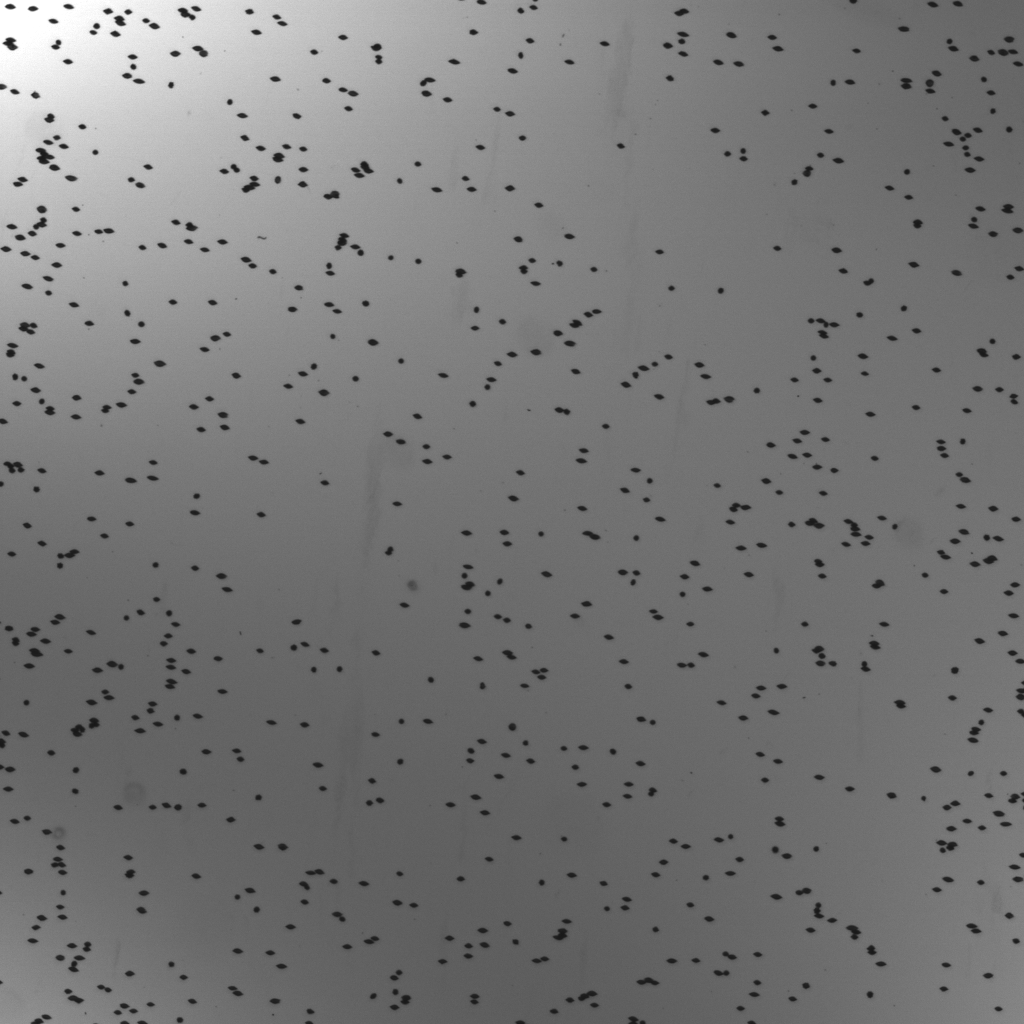
\includegraphics[width=150px, height=150px]{horizontal_0.png}}}
        \qquad
        \subfloat[\centering]{{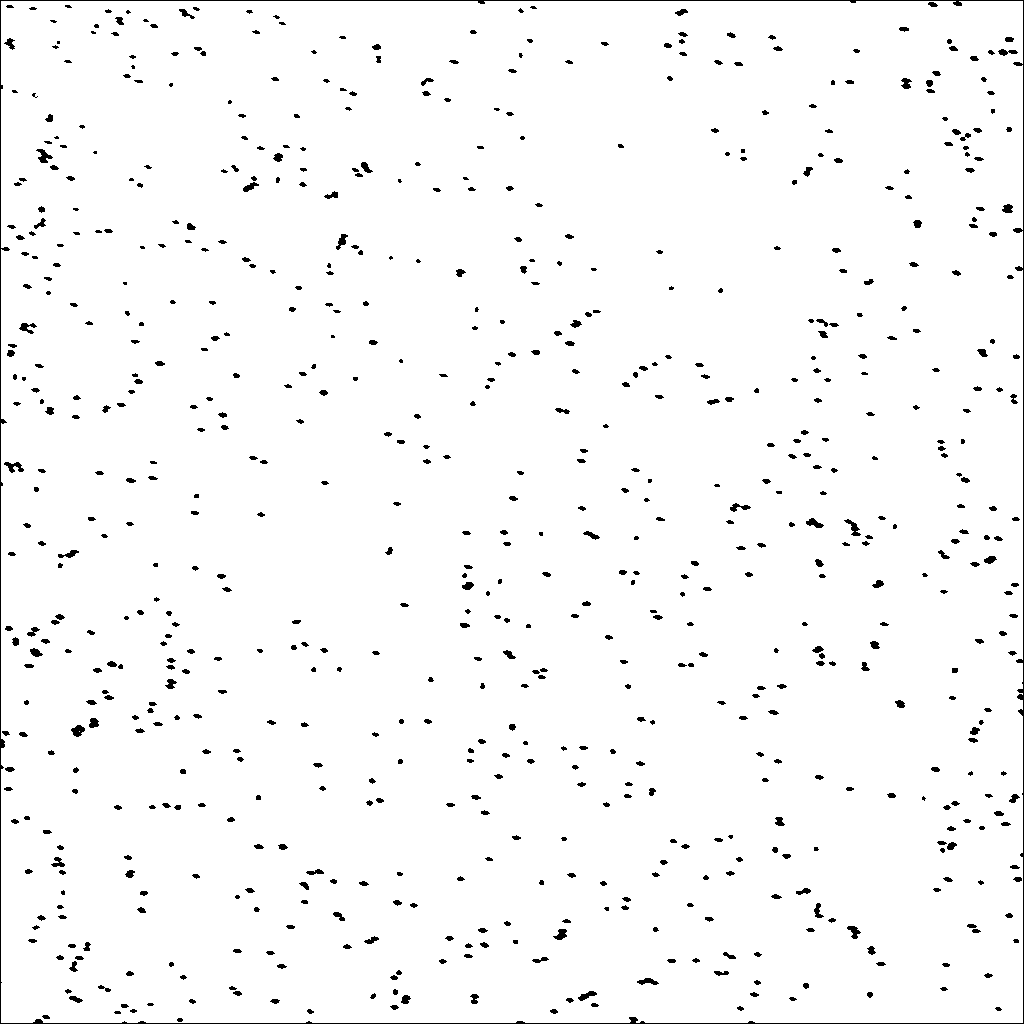
\includegraphics[width=150px, height=150px]{preview.png}}}
        \caption
        {
            (\textit{Opracowanie własne}) Przykład operacji binaryzacji.\\
            (a) Obraz wynikowy (powstały po podzieleniu obrazu głównego)\\
            (b) Obraz powstały w wyniku procesu binaryzacji obrazu wynikowego.
            Parametr binaryzacji odczytywany jest z pliku ``recipe.json'', który zapisany jest w sposób jaki pokazano na rysunku \ref{przykladowepliki}(b).
        }
    \end{figure}
    \subsection{Przykład Otwarcia}
    \begin{figure}[H]
        \centering
        \subfloat[\centering]{{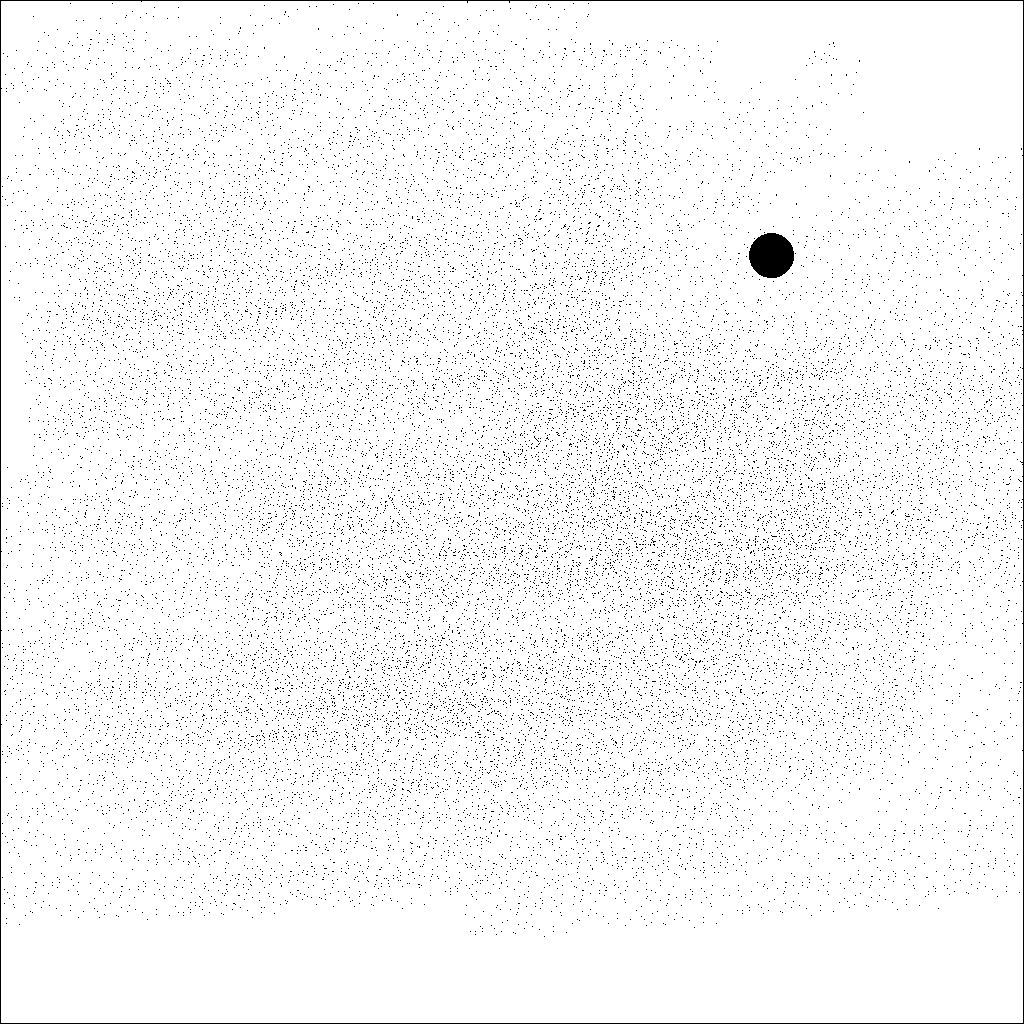
\includegraphics[width=150px, height=150px]{preview-otwarcie-start.png}}}
        \qquad
        \subfloat[\centering]{{
\includegraphics[width=150px, height=150px]{preview-otwarcie-end.png}}}
        \caption
        {
            (\textit{Opracowanie własne}) Przykład operacji otwarcia.\\
            (a) Przykładowy obraz zawierający jeden duży obiekt oraz szum.\\
            (b) Obraz powstały w wyniku operacji otwarcia na obrazie przykładowym elementem strukturalnym o rozmiarach 3 na 3.
            Szum został usunięty.
        }
    \end{figure}
    \subsection{Przykład Zamknięcia}
    \begin{figure}[H]
        \centering
        \subfloat[\centering]{{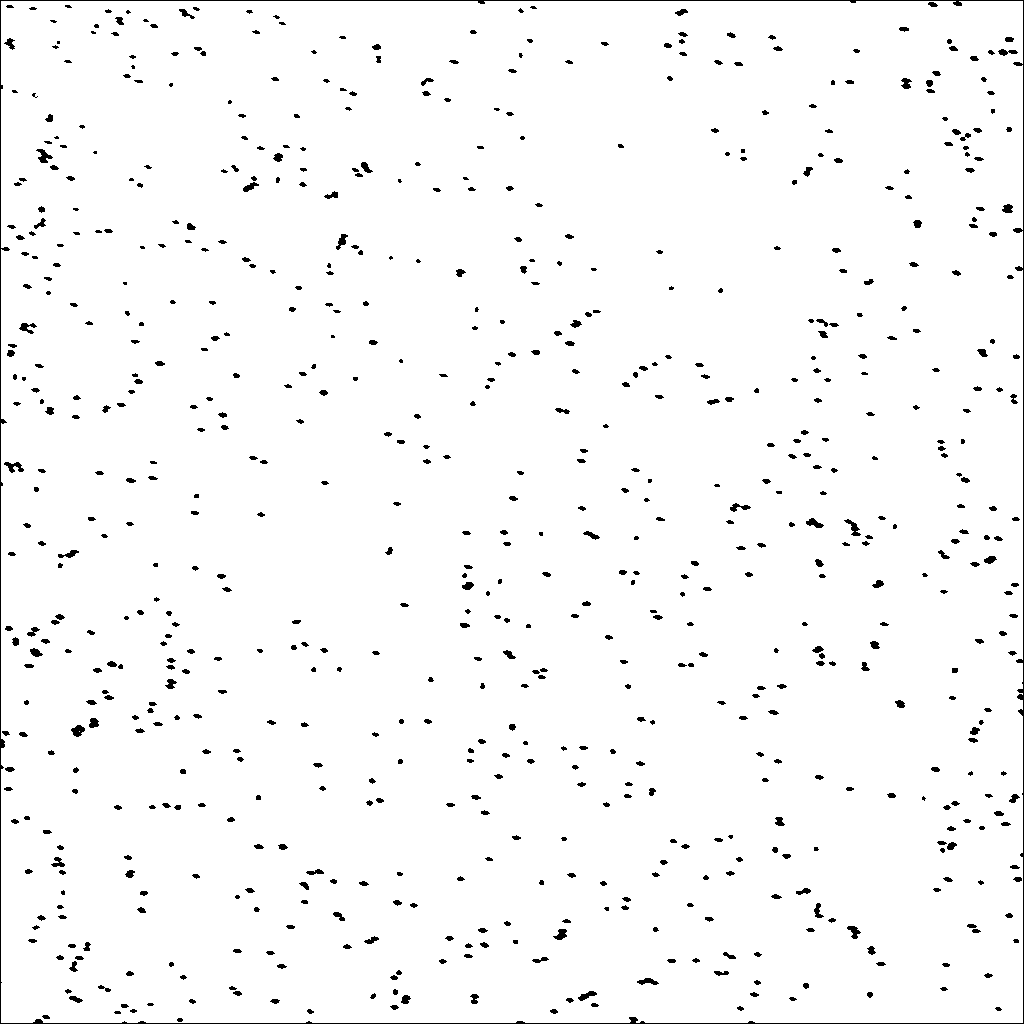
\includegraphics[width=150px, height=150px]{preview-zamkniecie-start.png}}}
        \qquad
        \subfloat[\centering]{{
\includegraphics[width=150px, height=150px]{preview-zamkniecie- end.png}}}
        \caption
        {
            (\textit{Opracowanie własne}) Przykład operacji zamknięcia.\\
            (a) Przykładowy obraz.\\
            (b) Obraz powstały w wyniku operacji zamknięcia na obrazie przykładowym elementem strukturalnym o rozmiarach 9 na 9.
            Niektóre obiekty zostały połączone i zwiększyły swoją powierzchnię.
        }
    \end{figure}
    \subsection{Przykład Dylatacji}
    \begin{figure}[H]
        \centering
        \subfloat[\centering]{{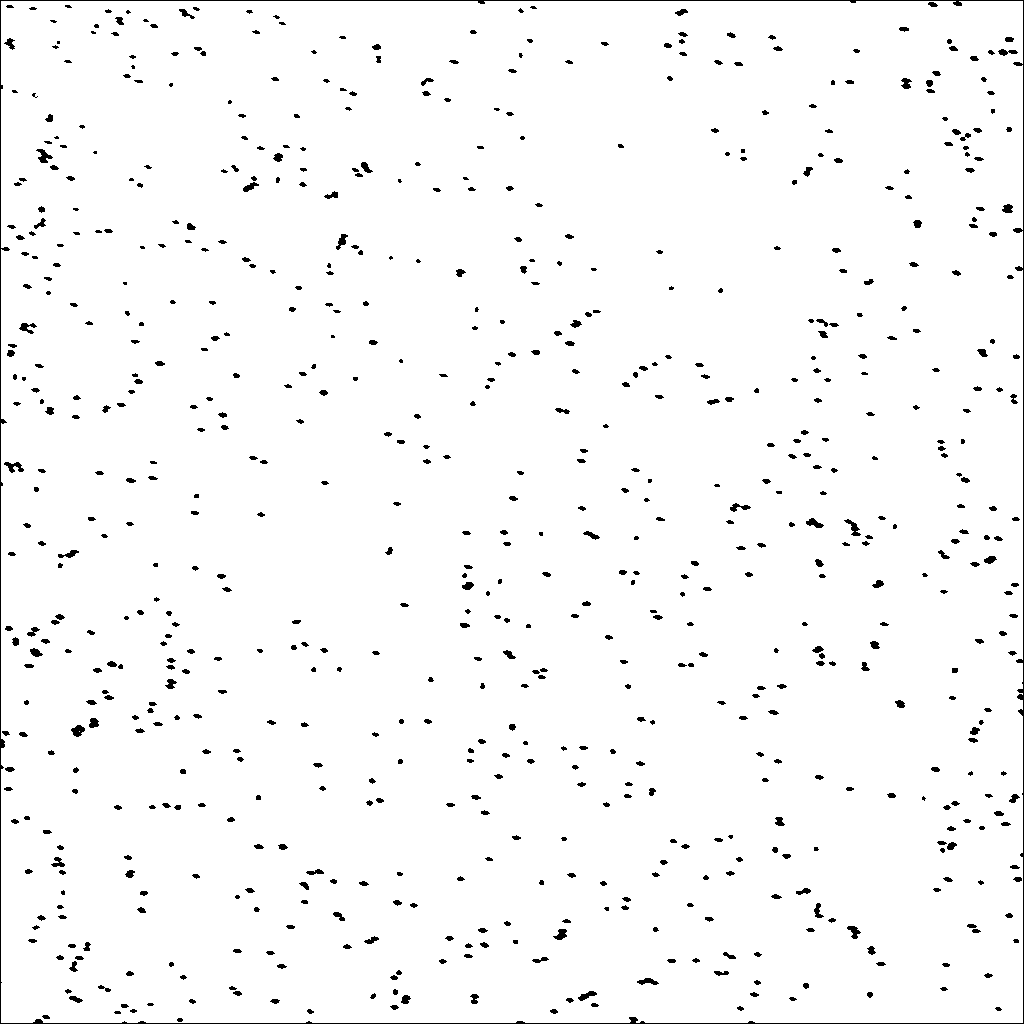
\includegraphics[width=150px, height=150px]{preview-dilation-start.png}}}
        \qquad
        \subfloat[\centering]{{
\includegraphics[width=150px, height=150px]{preview-dilation-end.png}}}
        \caption
        {
            (\textit{Opracowanie własne}) Przykład operacji dylatacji.\\
            (a) Przykładowy obraz.\\
            (b) Obraz powstały w wyniku operacji dylatacji na obrazie przykładowym elementem strukturalnym o rozmiarach 9 na 9.
            Wszystkie obiekty wyraźnie zwiększyły swoją powierzchnię.
        }
    \end{figure}
    \subsection{Przykład Erozji}
    \begin{figure}[H]
        \centering
        \subfloat[\centering]{{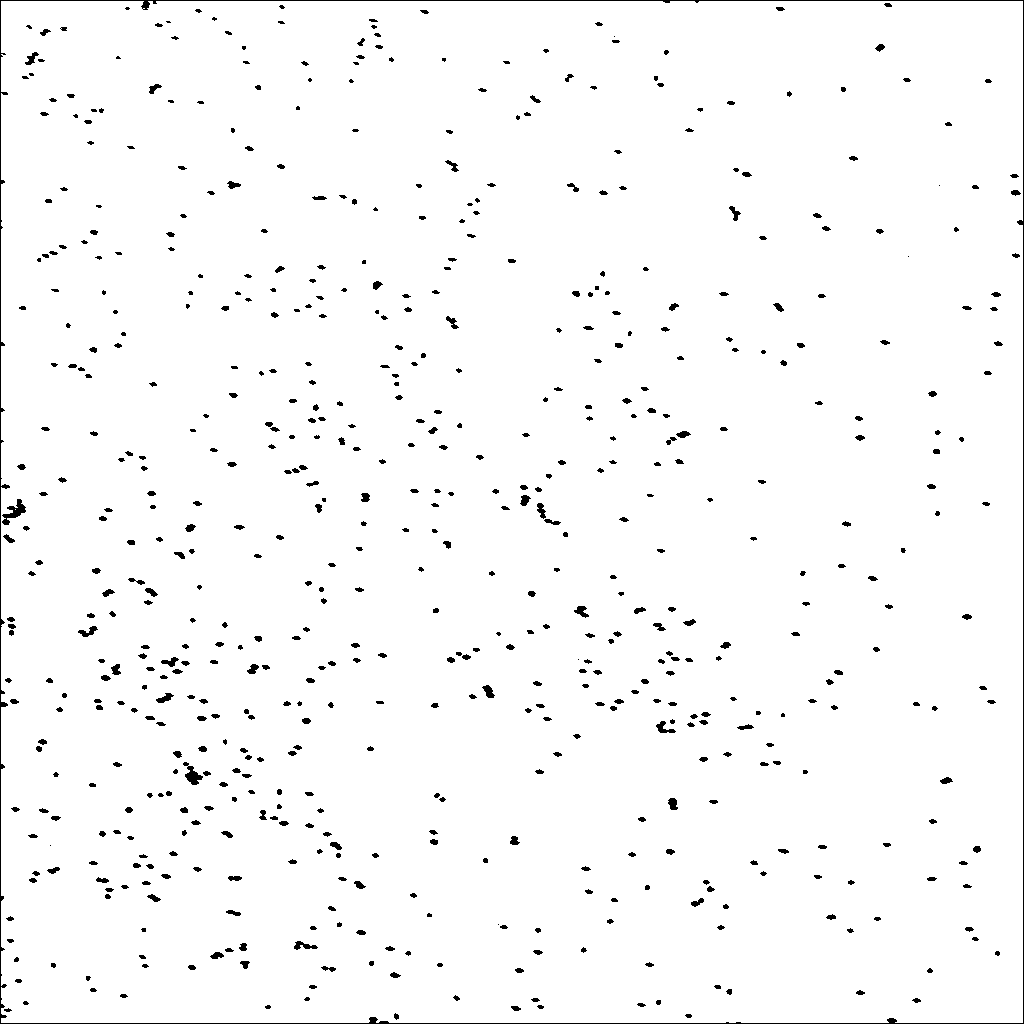
\includegraphics[width=150px, height=150px]{preview-erosion-start.png}}}
        \qquad
        \subfloat[\centering]{{
\includegraphics[width=150px, height=150px]{preview-erosion-end.png}}}
        \caption
        {
            (\textit{Opracowanie własne}) Przykład operacji erozji.\\
            (a) Przykładowy obraz.\\
            (b) Obraz powstały w wyniku operacji erozji na obrazie przykładowym elementem strukturalnym o rozmiarach 3 na 3.
            Wszystkie obiekty wyraźnie zmniejszyły swoją powierzchnię, niektóre całkiem zniknęły.
        }
        \label{erozjaex}
    \end{figure}
    \subsection{Przykład Etykietowania}
    \begin{figure}[H]
        \centering
        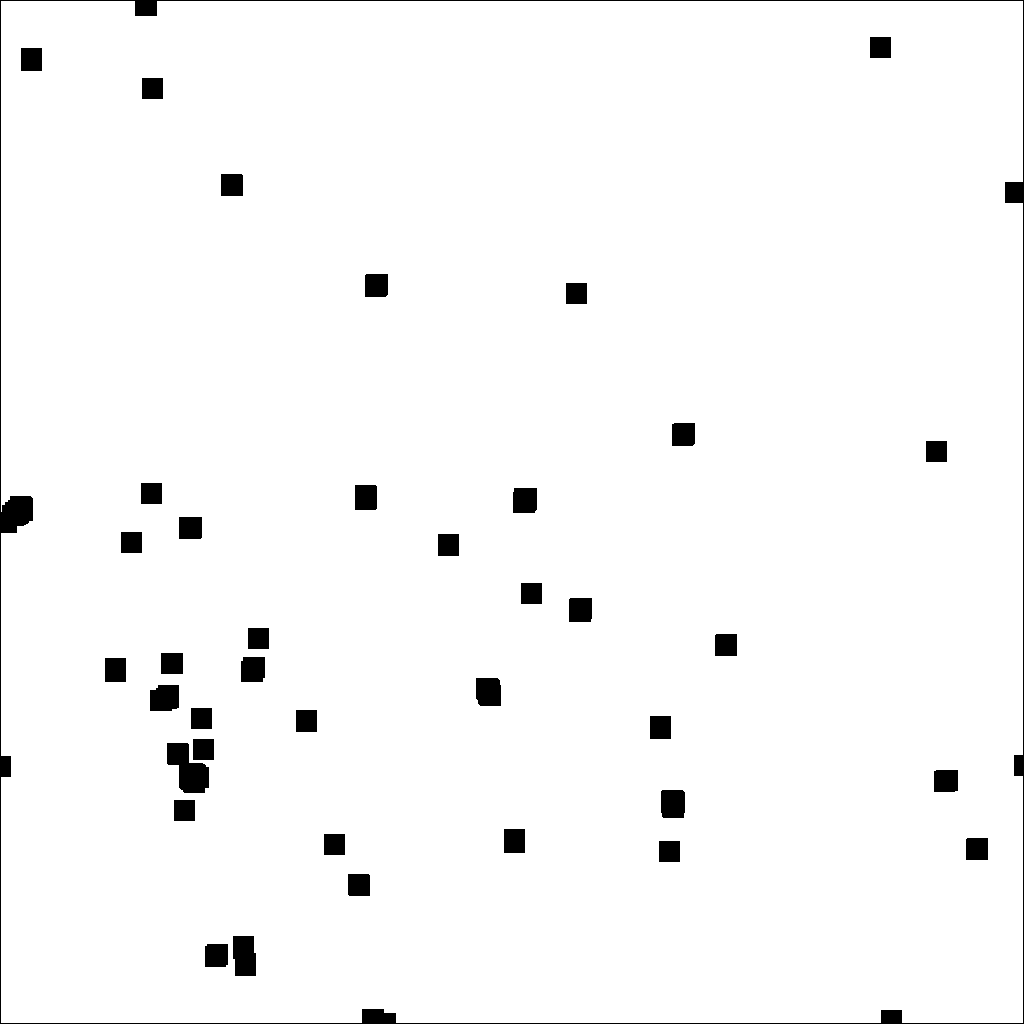
\includegraphics[width=300px]{label-example.png}
        \caption
        {
            (\textit{Opracowanie własne}) Przykładowy obraz.
        }
    \end{figure}
    {
        \label{przygotowaniekataloguglownego}
        \Large
        \justifying
        \quad
        Przykładowy obraz zawiera 44 elementy, co zostało policzone ręcznie.
        Za pomocą matematycznych funkcji na pole prostokąta przybliżona suma pól powierzchni obiektów została wyestymowana na 26000 pikseli.
    }
    \begin{figure}[H]
        \centering
        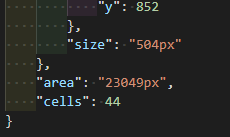
\includegraphics{wynik-koniec-koniec.png}
        \caption{\textit{(Opracowanie własne)} Zapis z pliku ``results.json''.}
        \label{konieckoniec}
    \end{figure}
    {
        \label{przygotowaniekataloguglownego}
        \Large
        \justifying
        \quad
        Zapis z pliku ``results.json'' wskazuje dużo dokładniejszą sumę pól powierzchni wszystkich obiektów.
        Błąd wynosi mniej niz 12\%, przez co obydwa wyniki dałyby miarodajną ocenę adhezji składników komórkowych.
        Z prostych przyczyn lepiej jednak skorzystać z dokładniejszego wyniku.
        Aby obliczyć adhezję potrzebujemy jeszcze ilości wszystkich pikseli na obrazie.
        Wszystkie obrazy wynikowe (powstałe w wyniku podzielenia obrazu głównego) mają rozmiar $1024 \times 1024$ pikseli,
        stąd ich suma wynosi $1048576$ pikseli.
        Ocena adhezji: $23049 / 1048576 = 0,022$.
        Porównanie wyników z kolejnych obrazów ukazuje zmianę adhezji.
        Ocena adhezji to jasna informacja na temat tego jak wiele komórek znalazło się na obrazie.
    }
    \newpage
    \section{Wnioski}
    {
        \Large
        \justifying
        \quad
        Opracowana biblioteka pozwala w łatwy sposób tworzyć spersonalizowane procesy przetwarzania obrazów cyfrowych.
        Algorytmy działają szybko i poprawnie.
        Istniejące mechanizmy wewnątrz biblioteki pozwalają na podgląd postepu zachodzących procesów.
        Dzięki możliwości personalizacji procesu przetwarzania, poszczególne obrazy mogą mieć swój własny ``przepis''.
        Możemy w łatwy sposób pozbyć się szumu, zmienić próg względem, którego przebiega proces binaryzacji czy też dostosować jasność obrazu.
    }

    \vspace{0.5cm}

    {
        \Large
        \justifying
        \quad
        Wyniki zapisywane są starannie do plików, każdy przetwarzany obraz ma swój własny plik z wynikami.
        Dzięki temu możemy w prosty sposób odczytać informacje na temat tego, z jakich pikseli składa się dana komórka.
        Każdy piksel opisany został współrzędnymi $x$ oraz $y$.
        Przez co łatwo możemy zlokalizować go na obrazie wynikowym.
        Każdy plik z wynikami ma na końcu informacje o sumie pól powierzchni wszystkich komórek na obrazie, a także ile takich komórek zostało znalezionych.
    }

    \vspace{0.5cm}

    {
        \Large
        \justifying
        \quad
        Wybór językia C++ okazał się być mieczem obosiecznym.
        Dzięki niemu mamy bardzo sprawnie działające algorytmy, a przez niego kod źródłowy rozrósł się tak bardzo, że został dołączony jako załącznik do tej pracy.
    }

    \vspace{0.5cm}

    {
        \Large
        \justifying
        \quad
        Opracowana biblioteka testowana była w warunkach rzeczywistych tzn. takich, w których przyjdzie jej pracować.
        Pozwoliło to na poprawienie jej działania i usprawnienia niektórych funkcji i klas.
        Dzięki temu wiemy, że wyzwania, które na nią czekają nie będą większe, niż to z czym do tej pory przyszło jej się zmagać.
    }

    \vspace{0.5cm}

    {
        \Large
        \justifying
        \quad
        Stworzona aplikacja okienkowa pozwala na wykorzystanie części możliwości jakie niesie ze sobą biblioteka ``BIA.Core''.
        Dobrym pomysłem na przyszłość byłoby rozwijanie tej aplikacji, aby mogła wykorzystać wszystkie funkcjonalności jakie wspomniana wcześniej biblioteka posiada.
        Jednak przenoszenie funkcjonalności z języki C++ do C\# za pomocą C++/CLI jest bardzo czasochłonne.
    }

    \newpage
    \section{Podsumowanie}
    {
        \Large
        \justifying
        \quad
        Celem niniejszej pracy było stworzenie biblioteki zajmującej się analizą i przetwarzaniem obrazów cyfrowych.
        Biblioteka miała za zadanie ocenę adhezji komórek krwi, co robi w stopniu zadawalającym wykorzystując szybkie algorytmy oraz proces personalizacji przetwarzania obrazów.
        Dzięki zautomatyzowaniu procesów, które do tej pory były wykonywane ręcznie spełnia również drugi cel - usprawnienie pracy ludzi.
        Utrzymywany kontakt z osobami, które będą z niej korzystały pozwoliło na stworzenie jej w wygodny do użycia sposób.
    }

    \vspace{0.5cm}

    {
        \Large
        \justifying
        \quad
        Tworząc bibliotekę ``BIA.Core'' nie brano pod uwagę jej zastosowania na szerszą skalę.
        Została napisana w jednym konkretnym celu i do jednego konkretnego zadania.
        Rozwijanie jej jednak mogłoby okazać się dobrym pomysłem, gdyż część biblioteki napisana jest w sposób pozwalający na wykorzystanie jej w ogólnych przypadkach.
    }

    \vspace{0.5cm}

    {
        \Large
        \justifying
        \quad
        Czasochłonność tworzenia oprogramowania, które za pomocą C++/CLI łączy funkcjonalności C++ oraz C\# jest trudna do wyestymowania.
        Nauka jaka z tego płynie na pewno zostanie ze mną na zawsze.
        Architektura oprogramowania jaką zastosowano w tym rozwiązaniu nie jest zbyt optymalna pod względem rozwoju i utrzymania kodu.
    }

    \newpage
    \section{Bibliografia}
    \begin{thebibliography}{9}

        \bibitem{msdocsmsbuild}
        Microsoft Docs
        \textit{MSBuild}
        \url{https://docs.microsoft.com/en-us/visualstudio/msbuild/msbuild?view=vs-2019}\\
        Stan na dzień 05/12/2020

        \bibitem{Molecular Biology of the Cell. 4th edition}
        Alberts B, Johnson A, Lewis J
        \textit{Molecular Biology of the Cell. 4th edition}
        New York, Garland Science, 2002

        \bibitem{adhezja}
        \textit{Wikipedia}
        \url{https://en.wikipedia.org/wiki/Adhesion#:~:text=Adhesion%20is%20the%20tendency%20of,be%20divided%20into%20several%20types}\\
        Stan na dzień 30/12/2020

        \bibitem{Encyclopedia of Graphics File Formats: The Complete Reference}
        James D. Murray, William VanRyper
        \textit{Encyclopedia of Graphics File Formats: The Complete Reference}
        O'Reilly Media, Second Edition, 1996, strony 880-908

        \bibitem{Digital Image Processing Second Edition}
        Rafael C. Gonzalez, Richard E. Woods
        \textit{Digital Image Processing Second Edition}
        Prentice Hall, Upper Saddle River, New Jersey 2002, strony 81, 523-532

        \bibitem{aipocwiki}
        \textit{Cyforwe przetwarzanie obrazów binarnych}
        \url{https://pl.wikipedia.org/wiki/Cyfrowe_przetwarzanie_obraz%C3%B3w_binarnych}\\
        Stan na dzień 30/12/2020

        \bibitem{LibTIFF tutorial}
        \textit{LibTIFF - Tutorial}
        \url{https://research.cs.wisc.edu/graphics/Courses/638-f1999/libtiff_tutorial.html}\\
        Stan na dzień 09/01/2021
    
        \bibitem{Program GIMP}
        \textit{Program GIMP}
        \url{https://www.gimp.org/}\\
        Stan na dzień 10/01/2021

        \bibitem{Program CMake}
        \textit{Program CMake}
        \url{https://www.cmake.org/}\\
        Stan na dzień 13/01/2021

        \bibitem{Biblioteka LibTIFF}
        \textit{Biblioteka LibTIFF}
        \url{http://www.libtiff.org/}\\
        Stan na dzień 30/12/2020

        \bibitem{VS2019}
        \textit{Program Visual Studio 2019}
        \url{https://visualstudio.microsoft.com/vs/}\\
        Stan na dzień 10/01/2021

        \bibitem{LaTeX}
        \LaTeX \space
        \url{https://www.latex-project.org/}\\
        Stan na dzień 10/01/2021

        \bibitem{VSCode}
        \textit{Program Visual Studio Code}
        \url{https://code.visualstudio.com/}\\
        Stan na dzień 10/01/2021

        \bibitem{.NET Framework}
        \textit{What is .NET Framework?}
        \url{https://dotnet.microsoft.com/learn/dotnet/what-is-dotnet-framework}\\
        Stan na dzień 09/01/2021

        \bibitem{nlohmann.json 3.9.1}
        \textit{nlohmann.json 3.9.1}
        \url{https://github.com/nlohmann/json}\\
        Stan na dzień 30/01/2021

        \bibitem{OpenMP 5.1}
        \textit{OpenMP 5.1}
        \url{https://www.openmp.org/}\\
        Stan na dzień 14/02/2021

        \bibitem{Building LibTiff}
        \textit{LibTIFF - Building the Software Distribution}
        \url{https://libtiff.gitlab.io/libtiff/build.html}\\
        Stan na dzień 09/01/2021

    \end{thebibliography}
    \newpage
    \listoffigures
\end{document}